\documentclass[serif ,mathserif ,professionalfont,hyperref={pdfpagelabels=false}]{beamer}
%\usepackage{lmodern}
\usepackage{exscale}
\usepackage{amsmath}
\usepackage{graphicx}
%\usepackage{mathptmx} % seems something to do with the font
\usepackage{helvet}
\usepackage{tcolorbox}
\usepackage{textpos}
\usepackage{xargs}
\usepackage{tikz}
\usepackage{amssymb}
\usepackage[]{algorithm2e}
\usepackage{pxfonts}
\usepackage{eulervm}
\usepackage[miktex]{gnuplottex} % for MiKTeX,`pdflatex -shell-escape`
                                % enabled
\usepackage[export]{adjustbox}
\usepackage{cite}
%\usepackage{gnuplottex} I have used this line to compile on TeXLive 2013
%\usepackage[pdftex,dvipsnames]{xcolor}
%\usepackage[colorinlistoftodos,prependcaption,textsize=tiny]{todonotes}
\usepackage{mathtools}
\DeclareMathOperator*{\argmin}{argmin}
\DeclareMathOperator*{\argmax}{argmax}

\renewcommand{\familydefault}{helvetica}
%\renewcommand{\labelitemi}{$\bluesquare$}
\newcommand{\labelitemi}{\textbf{\ding{192}}}
\newcommand{\localtextbulletone}{\textcolor{gray}{\raisebox{.45ex}{\rule{.6ex}{.6ex}}}}
\newcommand\norm[1]{\left\lVert#1\right\rVert}
\renewcommand{\labelitemi}{\localtextbulletone}
%\renewcommand\mathfamilydefault{\mathnormal}
%\renewcommand{\theequation}{\thechapter--\arabic{equation}} % for
                                % equation number style



\DeclareMathOperator{\dom}{dom}
\def\gdw{\mathrel{{>}\mkern-13mu{<}}}

\setbeamertemplate{itemize items}[square]


\usetheme{Frankfurt}
\setbeamercolor{section in head/foot}{fg=white, bg=blue!20!black!90}


%% commands definitions for
\newcommand\mynew{andyandyandy}

%% end of the definition of commands

%%% block definition
\newenvironment<>{redblock}[1]{%
  \setbeamercolor{block title}{fg=white,bg=red!75!black!65}%
  \setbeamercolor{block body}{fg=red!40!black!70,bg=red!60!black!20}%

  \begin{block}#2{#1}}{\end{block}}
\newenvironment<>{blueblock}[1]{%
  \setbeamercolor{block title}{fg=white,bg=blue!75!black!65}%
  \setbeamercolor{block body}{fg=black,bg=blue!60!black!20}%
  \begin{block}#2{#1}}{\end{block}}

\newenvironment<>{greyblock}[1]{%
  \setbeamercolor{block title}{fg=white,bg=black!75}%
  \setbeamercolor{block body}{fg=black,bg=black!40}%
  \begin{block}#2{#1}}{\end{block}}

\newenvironment<>{greenblock}[1]{%
  \setbeamercolor{block title}{fg=white,bg=green!75!black!65}%
  \setbeamercolor{block body}{fg=black,bg=green!60!black!20}%
  \begin{block}#2{#1}}{\end{block}}
%%% Block definition


% for the note style
% \newcommandx{\unsure}[2][1=]{\todo[linecolor=red,backgroundcolor=red!25,bordercolor=red,#1]{#2}}
% \newcommandx{\change}[2][1=]{\todo[linecolor=blue,backgroundcolor=blue!25,bordercolor=blue,#1]{#2}}
% \newcommandx{\info}[2][1=]{\todo[linecolor=OliveGreen,backgroundcolor=OliveGreen!25,bordercolor=OliveGreen,#1]{#2}}
% \newcommandx{\improvement}[2][1=]{\todo[linecolor=Plum,backgroundcolor=Plum!25,bordercolor=Plum,#1]{#2}}
% \newcommandx{\thiswillnotshow}[2][1=]{\todo[disable,#1]{#2}}

%% configuration for the slids style
\makeatletter
\setbeamertemplate{footline}
{
  \leavevmode%
  \hbox{%
    \begin{beamercolorbox}[wd=.333333\paperwidth,ht=2.25ex,dp=1.6ex,center]{author in head/foot}%
      \usebeamerfont{author in
        head/foot}%
      \insertshortauthor\hspace{1em}\beamer@ifempty{Advanced
        Algorithms}{}{Advanced
        Algorithms}
    \end{beamercolorbox}%
    \begin{beamercolorbox}[wd=.333333\paperwidth,ht=2.25ex,dp=1.6ex,center]{title in head/foot}%
      \usebeamerfont{title in head/foot}\insertshorttitle
    \end{beamercolorbox}%
    \begin{beamercolorbox}[wd=.333333\paperwidth,ht=2.25ex,dp=1.6ex,right]{date in head/foot}%
      \usebeamerfont{date in head/foot}\insertshortdate{}\hspace*{2em}
      \insertframenumber{} / \inserttotalframenumber\hspace*{2ex}
    \end{beamercolorbox}}%
  \vskip0pt%
}
\makeatother

\author[\parbox{.2\paperwidth}{}]{Hu SiXing, Hakki Can Karaimer, Pan An, Philipp Keck}
\institute{National University of Singapore}
\title{Convex Optimization}

%% end of configuration




% \title{Convex Optimization}
% \author{Hu SiXing, Hakki Can Karaimer, Pan An, Philipp Keck}
% \date{\today}
\begin{document}

\begin{frame}
  \titlepage
\end{frame}


% \begin{frame}
%   % \frametitle{Table of contents}
%   % \tableofcontents
% %%% Local Variables:
%%% mode: latex
%%% TeX-master: t
%%% End:

%%  commands definition and some other definitions about stuffs
\newcommand\here{lalala}
%\newcommand\x{x_i}
%\newcommand\y{y_i
\newcommand\dis{\displaystyle }


\subsection{}
\begin{frame}
  \frametitle{Linear Regression Example}
  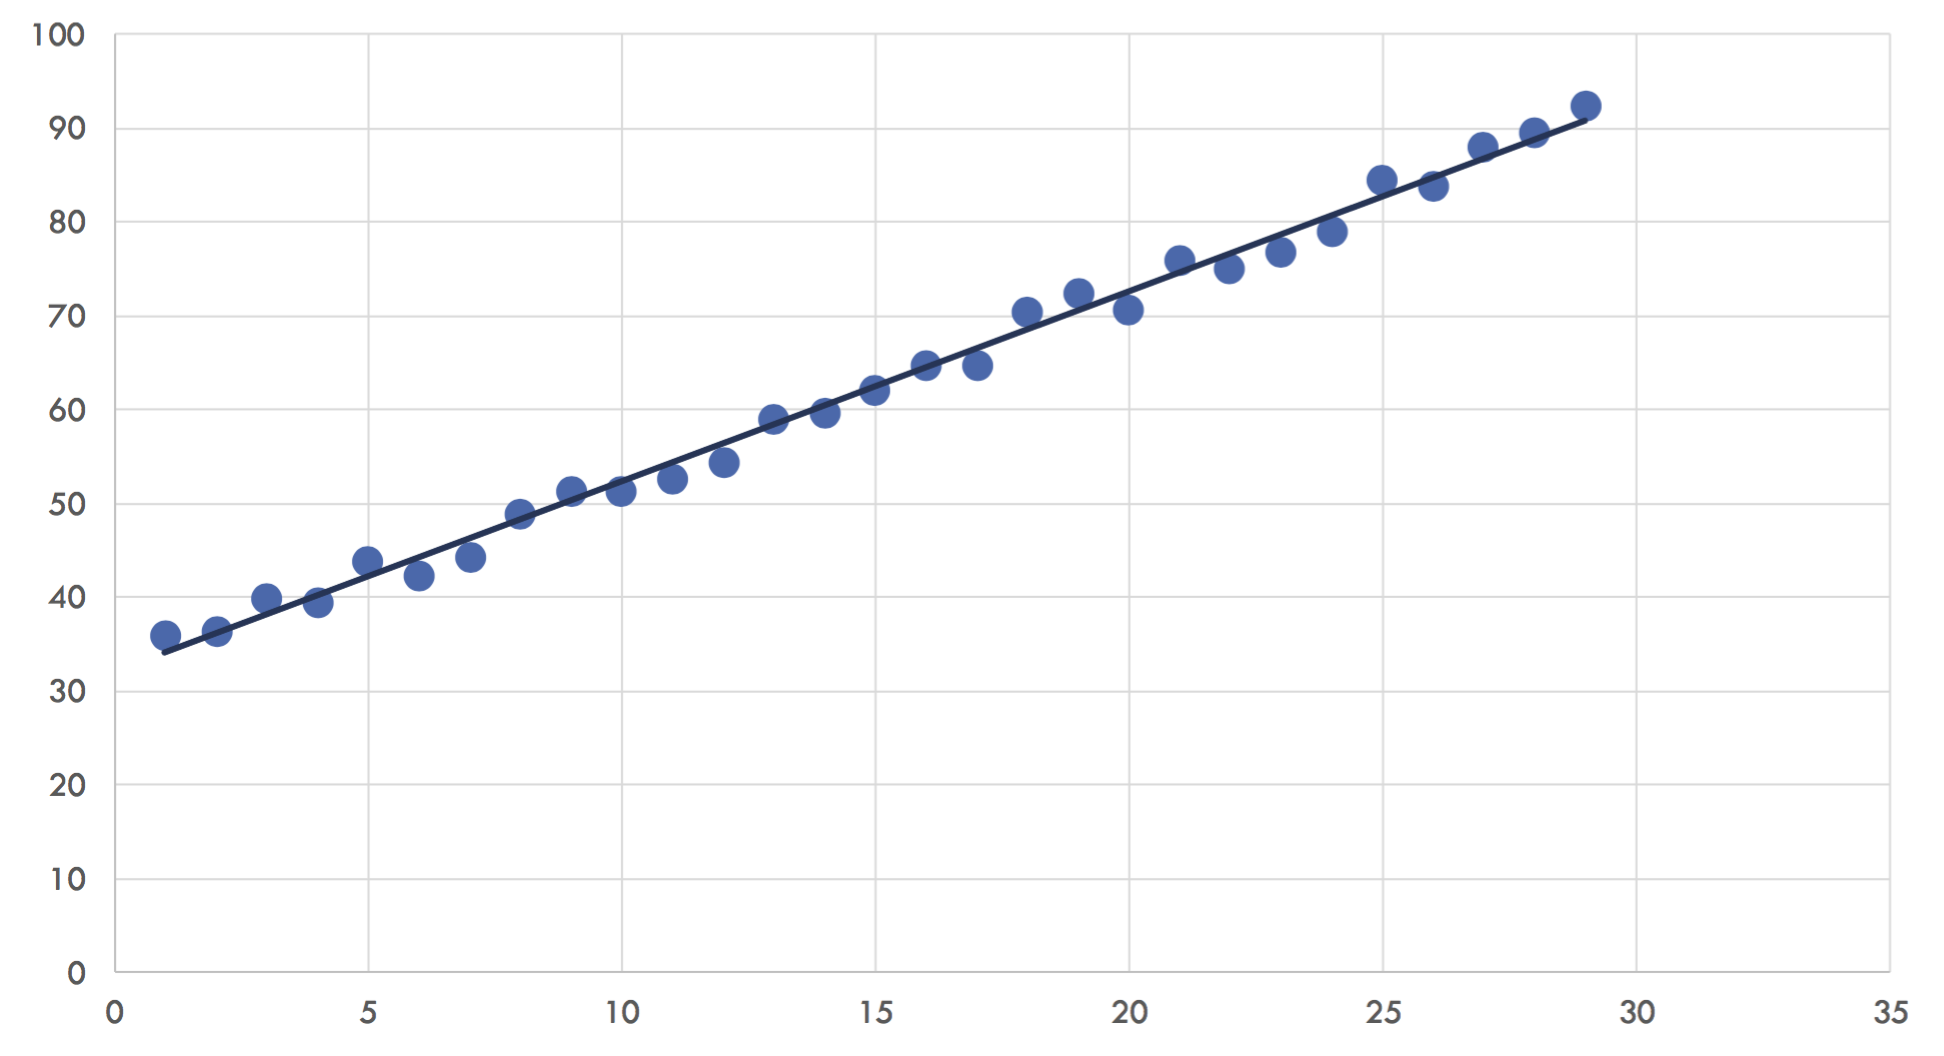
\includegraphics[scale=0.32]{pics/linear.png}

\end{frame}


\subsection{}
\begin{frame}
\frametitle{Ordinary Least Squares}

% 2 columns examples
\begin{columns}
  \begin{column}{0.6\textwidth}
    \begin{itemize}
    \item[] Input: points $(x_i, y_i)$
      \item[] Regression line: $y = mx + b$
\item[] Objective: $\displaystyle \min_{m, b} \sum_{i}(y_i - mx_i -b)^2$
    \end{itemize}
  \end{column}

  \begin{column}{0.5\textwidth}
    \begin{itemize}
    \item[] $(\vec{x_i}, y_i)$
    \item[] $y = \vec{w} \cdot \vec{x} + b$
    \item[] $\dis \min_{\vec{w}}\sum_{i}(y_i - \vec{w} \cdot \vec{x_i} -b)^2$
    \end{itemize}

  \end{column}
\end{columns}

\begin{itemize}
\item Easily Solved: $\vec{w}^*(X^TX)-X^T\vec{y}$
\item But what if $\dim\vec{x} $ is large?
\item What about other similar regressions?
\end{itemize}

\end{frame}

\subsection{}
\begin{frame}
\frametitle{Convex Optimization Problems}


\begin{itemize}
\item OrdinaryLinearRegression: $\dis \min_{\vec{w}}\sum_i(y_i -
  \vec{w} \cdot \vec{x_i})^2$
\item General: $\dis \min_xf(x)$ where $f(x)$ is convex
\item Set $C$ is convex $\Longleftrightarrow \forall x, y\in C, 0\le t
  \le 1: tx +(1 - t)y \in C$
\item Function $f : \mathbb{R}^n \rightarrow \mathbb{R}$ is convex if
  $\dom f$ is convex and $\exists x, y \in \dom f, 0\le t \le 1:$

\end{itemize}

\vspace{-4mm}

{\small
$$f(tx + (1 - t)y) \le tf(x) + (1 - t)f(y)$$
}

\vspace{-4mm}

\begin{columns}
  \begin{column}{0.5\textwidth}

\begin{itemize}
\item Unconstrained.
\end{itemize}

  \end{column}

  \begin{column}{0.5\textwidth}
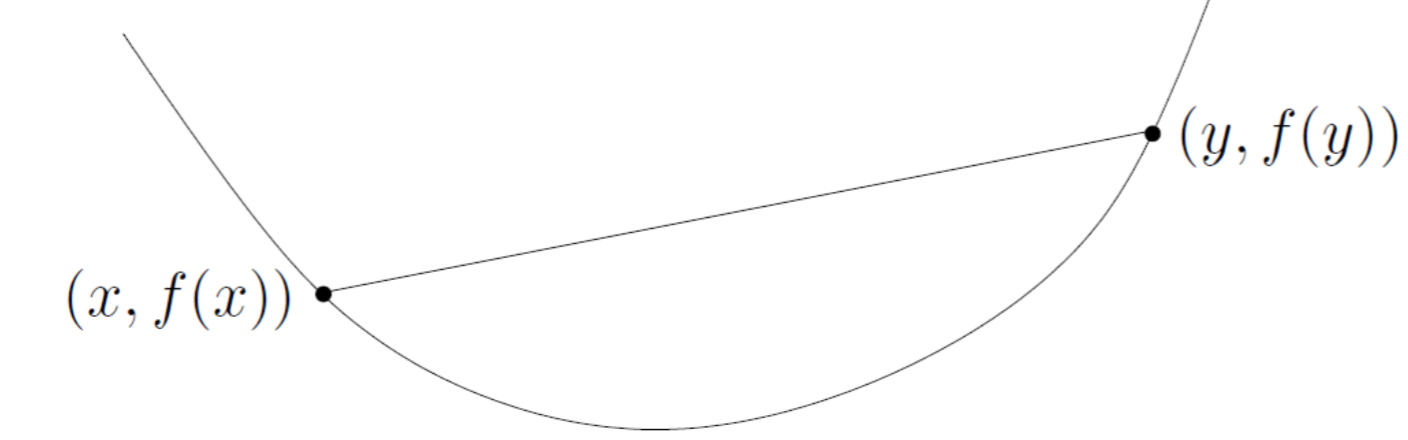
\includegraphics[scale=0.2]{pics/uncons.png}
  \end{column}
\end{columns}

\end{frame}

\subsection{}

\begin{frame}
  \frametitle{Outliers}
  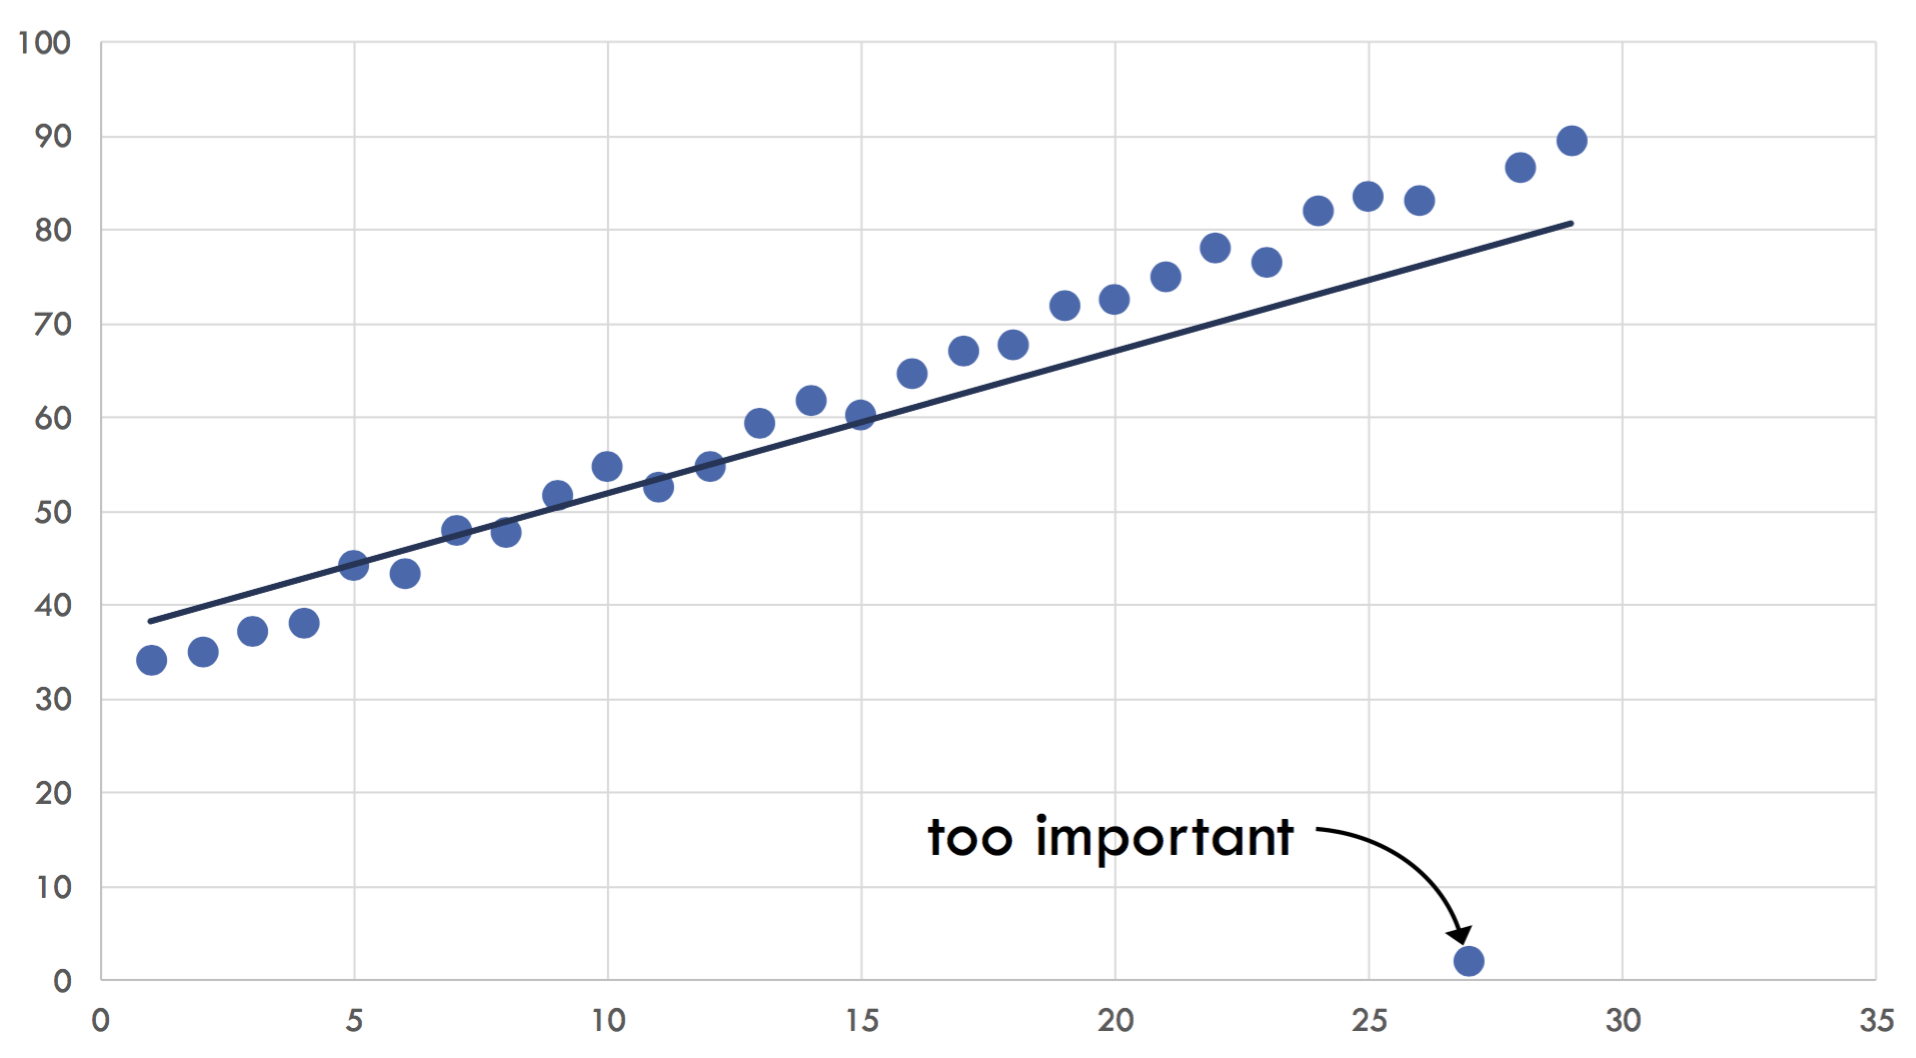
\includegraphics[scale=0.32]{pics/lpo.png}

\end{frame}

\subsection{}
\begin{frame}


  \frametitle{Outlier Penalty}

  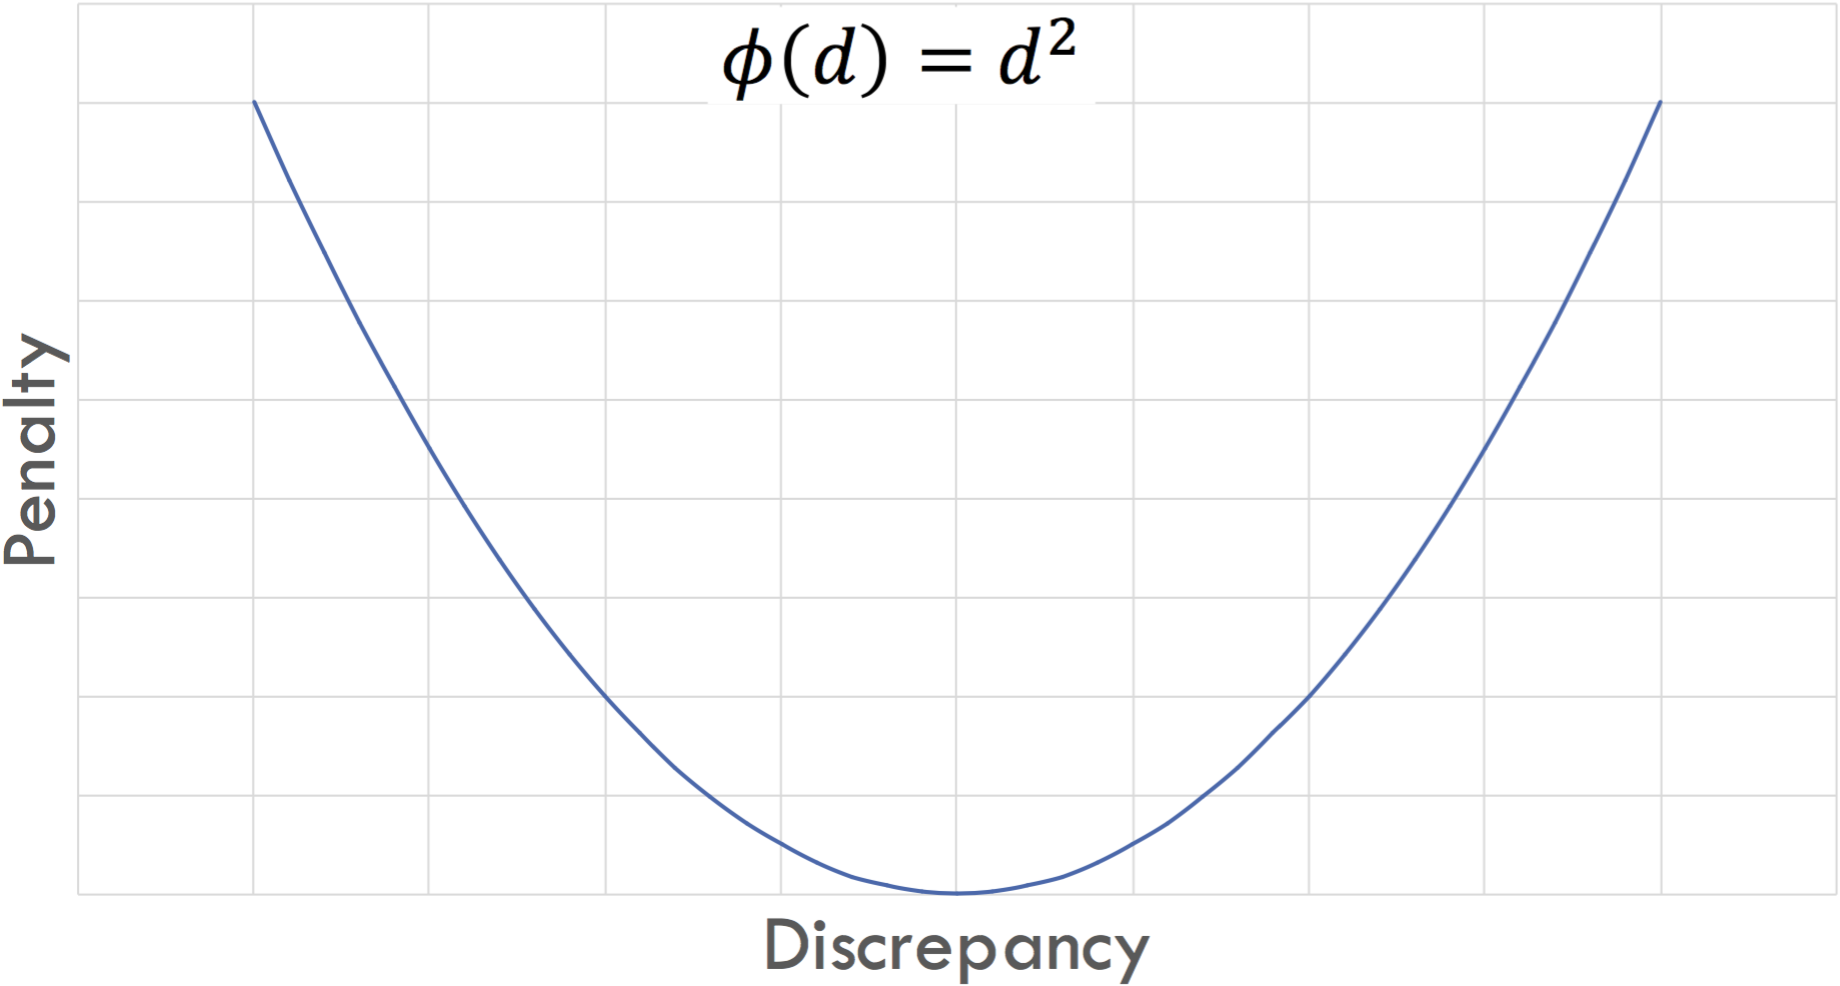
\includegraphics[scale=0.32]{pics/pen1.png}


\end{frame}

\begin{frame}
  \frametitle{Capped Penalty}
  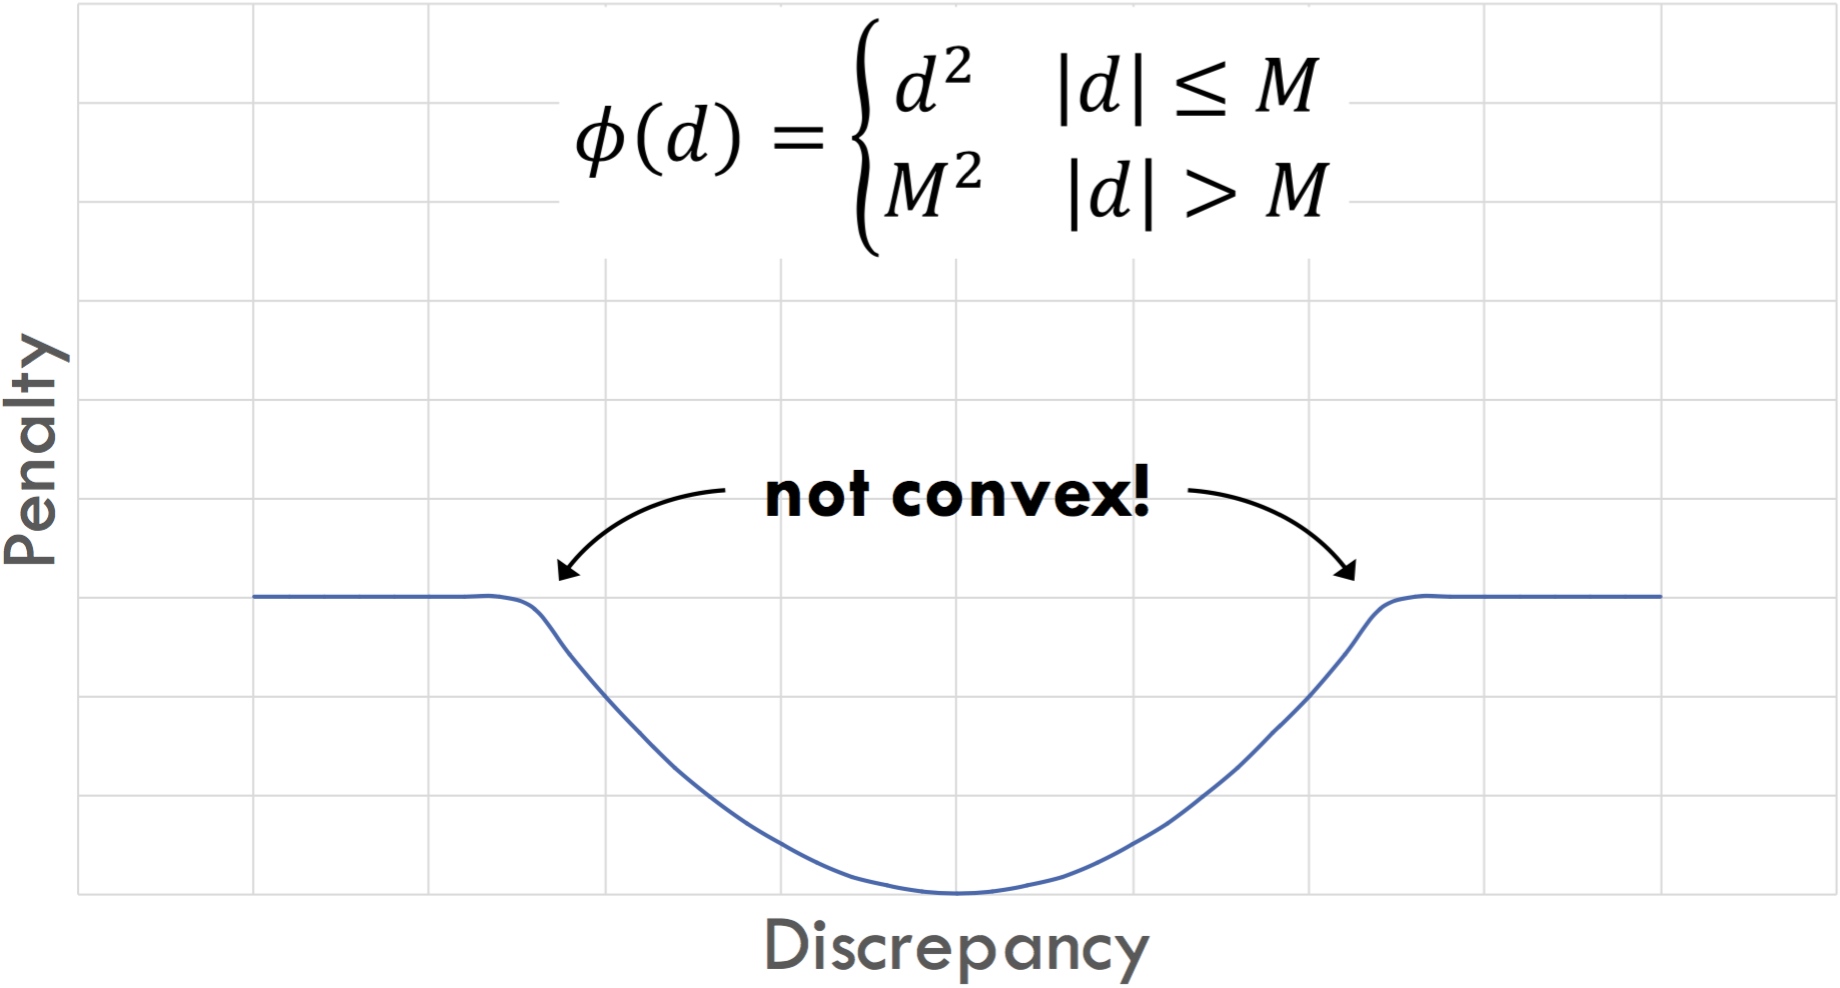
\includegraphics[scale=0.32]{pics/pen2.png}
\end{frame}

\begin{frame}
\frametitle{Huber Penalty Function}
  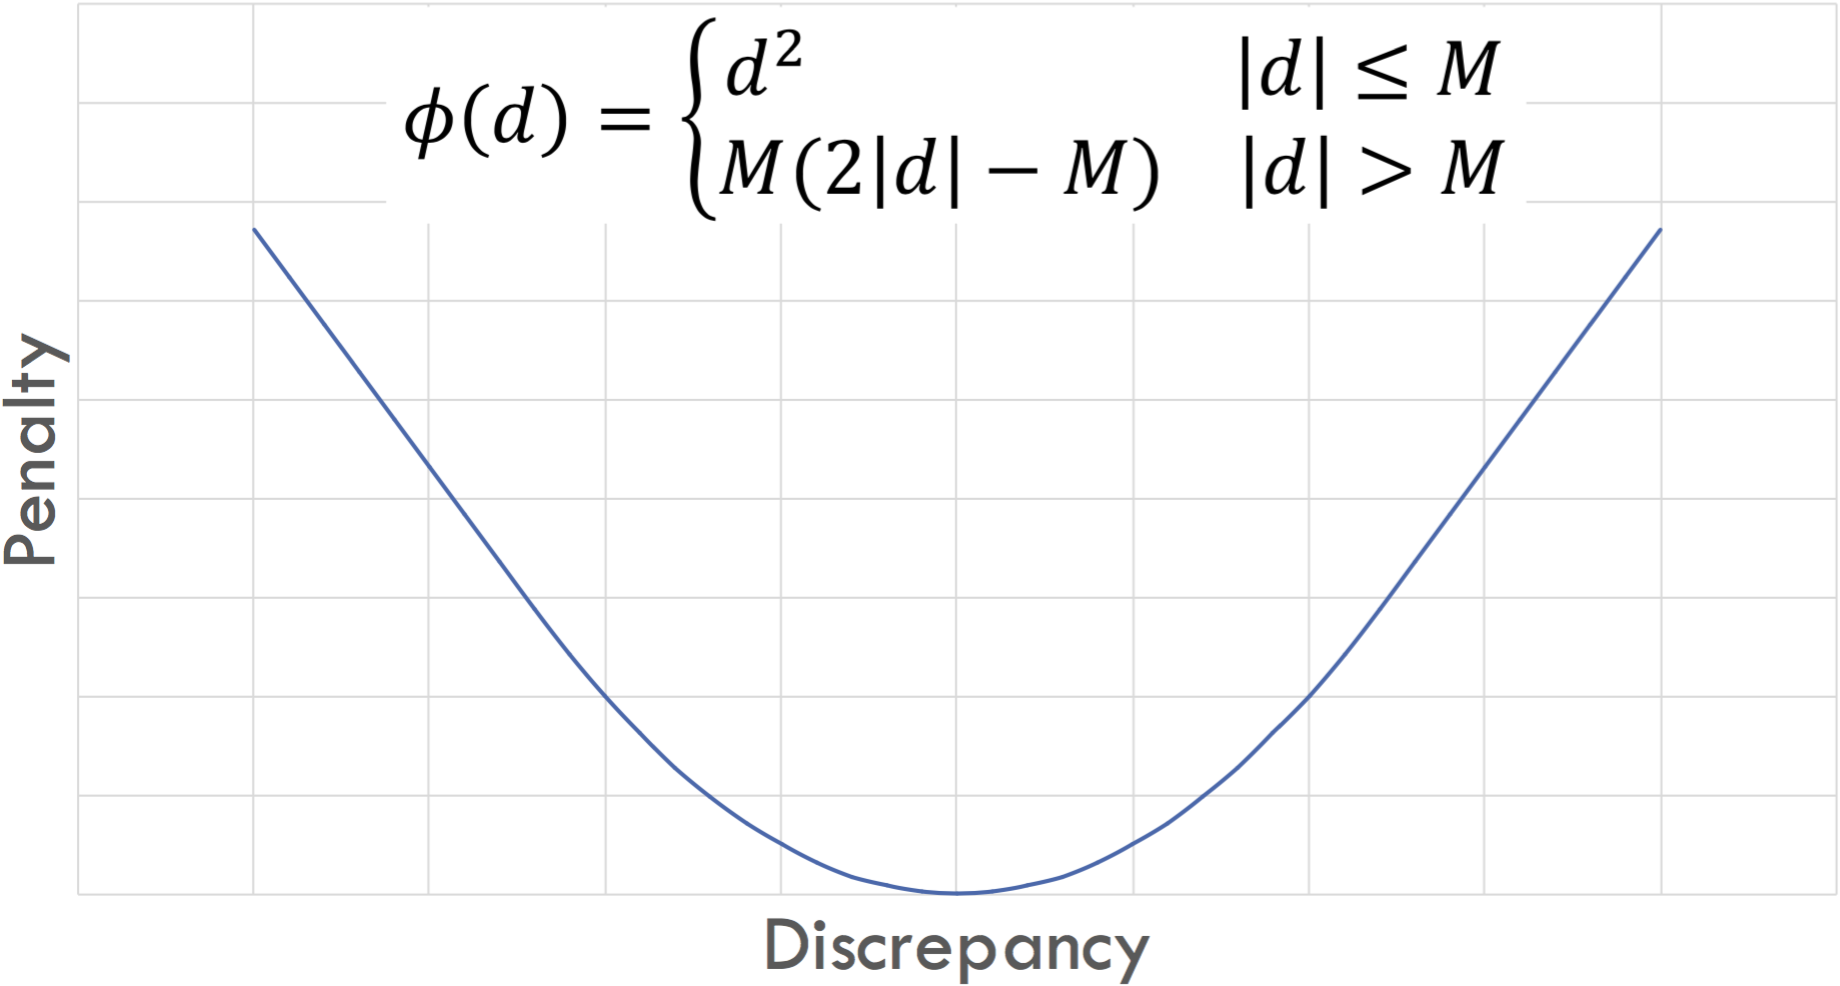
\includegraphics[scale=0.32]{pics/pen3.png}
\end{frame}

% \mynew
% \end{frame}


\section{Linear Regression}
%%% Local Variables:
%%% mode: latex
%%% TeX-master: t
%%% End:

%%  commands definition and some other definitions about stuffs
\newcommand\here{lalala}
%\newcommand\x{x_i}
%\newcommand\y{y_i
\newcommand\dis{\displaystyle }


\subsection{}
\begin{frame}
  \frametitle{Linear Regression Example}
  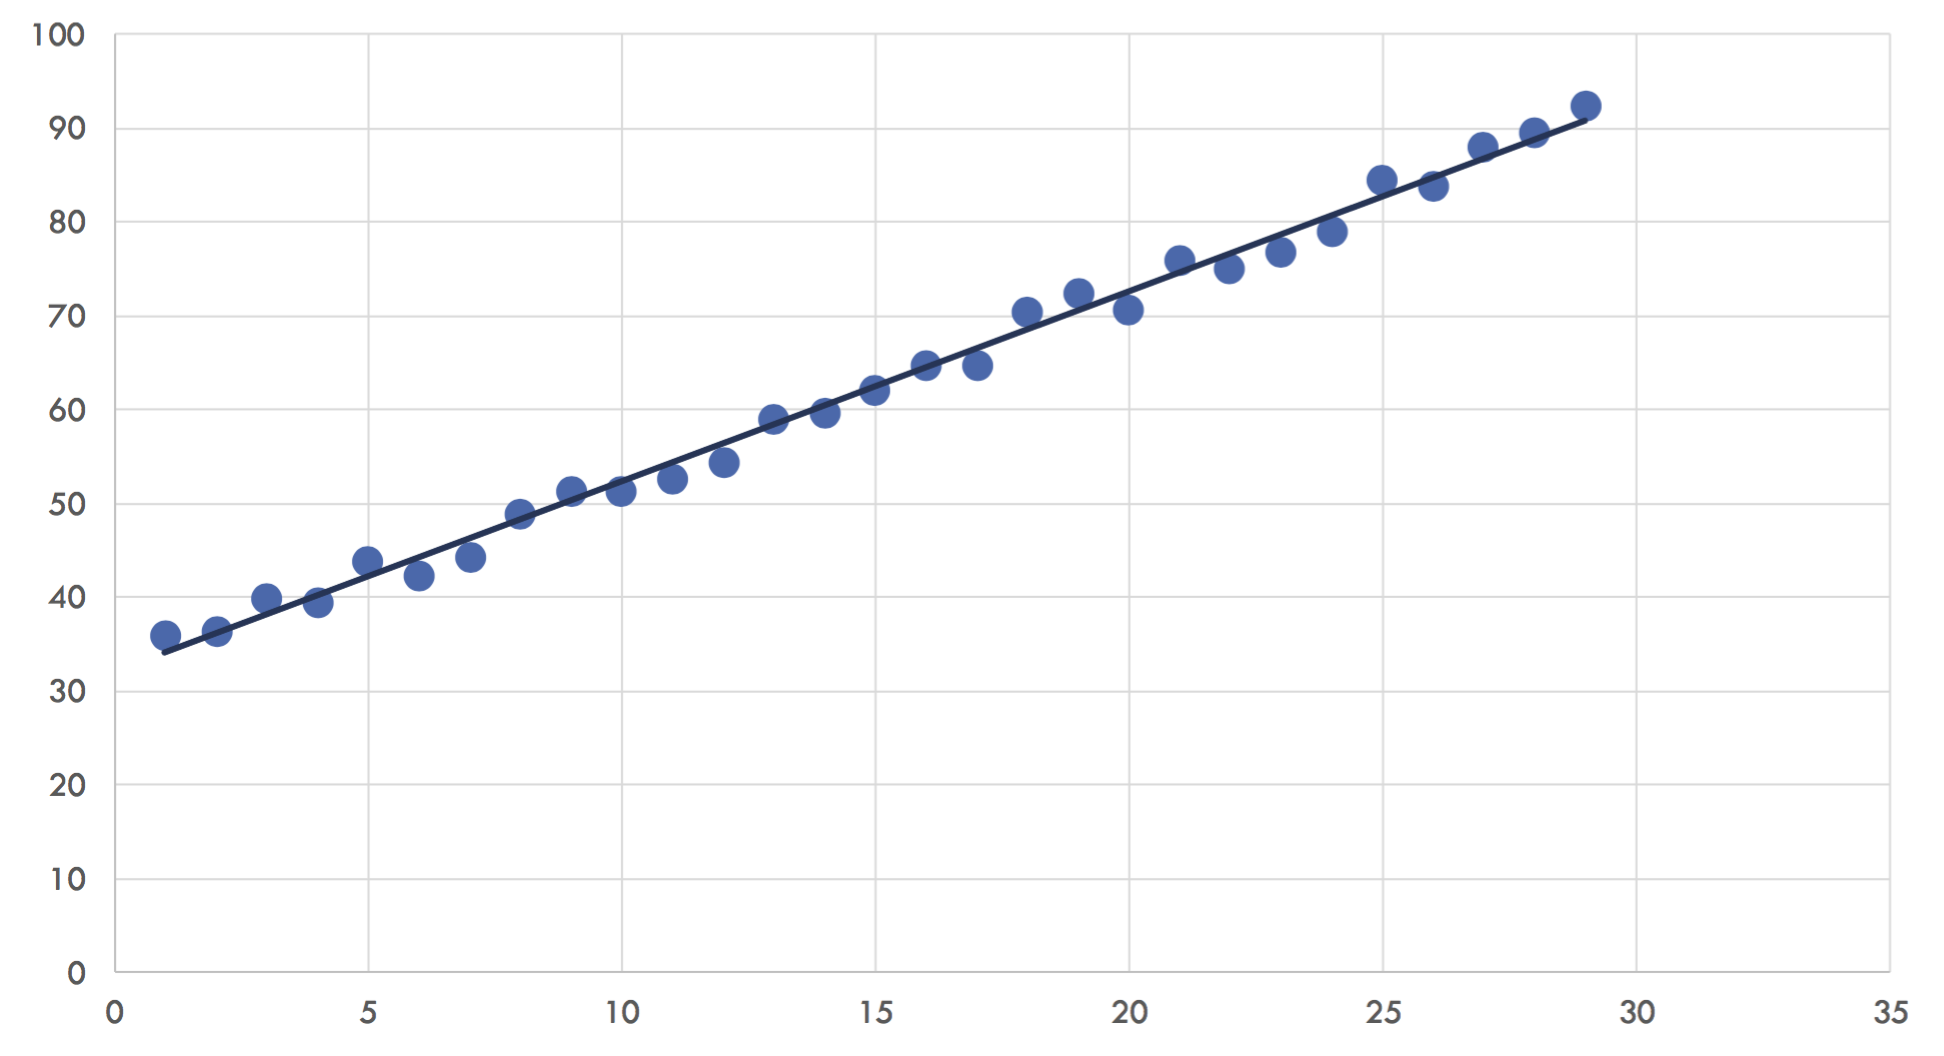
\includegraphics[scale=0.32]{pics/linear.png}

\end{frame}


\subsection{}
\begin{frame}
\frametitle{Ordinary Least Squares}

% 2 columns examples
\begin{columns}
  \begin{column}{0.6\textwidth}
    \begin{itemize}
    \item[] Input: points $(x_i, y_i)$
      \item[] Regression line: $y = mx + b$
\item[] Objective: $\displaystyle \min_{m, b} \sum_{i}(y_i - mx_i -b)^2$
    \end{itemize}
  \end{column}

  \begin{column}{0.5\textwidth}
    \begin{itemize}
    \item[] $(\vec{x_i}, y_i)$
    \item[] $y = \vec{w} \cdot \vec{x} + b$
    \item[] $\dis \min_{\vec{w}}\sum_{i}(y_i - \vec{w} \cdot \vec{x_i} -b)^2$
    \end{itemize}

  \end{column}
\end{columns}

\begin{itemize}
\item Easily Solved: $\vec{w}^*(X^TX)-X^T\vec{y}$
\item But what if $\dim\vec{x} $ is large?
\item What about other similar regressions?
\end{itemize}

\end{frame}

\subsection{}
\begin{frame}
\frametitle{Convex Optimization Problems}


\begin{itemize}
\item OrdinaryLinearRegression: $\dis \min_{\vec{w}}\sum_i(y_i -
  \vec{w} \cdot \vec{x_i})^2$
\item General: $\dis \min_xf(x)$ where $f(x)$ is convex
\item Set $C$ is convex $\Longleftrightarrow \forall x, y\in C, 0\le t
  \le 1: tx +(1 - t)y \in C$
\item Function $f : \mathbb{R}^n \rightarrow \mathbb{R}$ is convex if
  $\dom f$ is convex and $\exists x, y \in \dom f, 0\le t \le 1:$

\end{itemize}

\vspace{-4mm}

{\small
$$f(tx + (1 - t)y) \le tf(x) + (1 - t)f(y)$$
}

\vspace{-4mm}

\begin{columns}
  \begin{column}{0.5\textwidth}

\begin{itemize}
\item Unconstrained.
\end{itemize}

  \end{column}

  \begin{column}{0.5\textwidth}
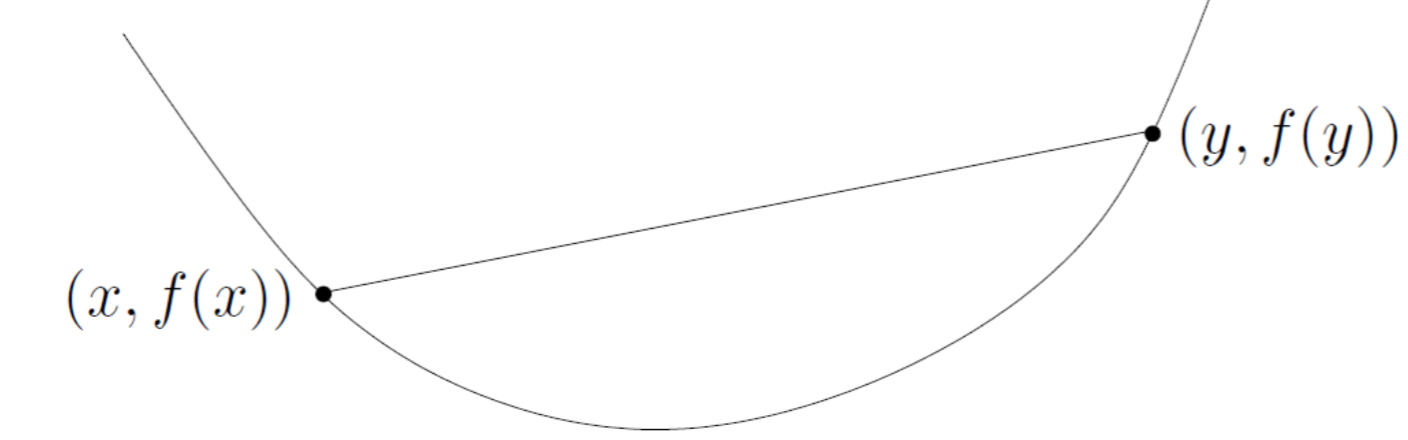
\includegraphics[scale=0.2]{pics/uncons.png}
  \end{column}
\end{columns}

\end{frame}

\subsection{}

\begin{frame}
  \frametitle{Outliers}
  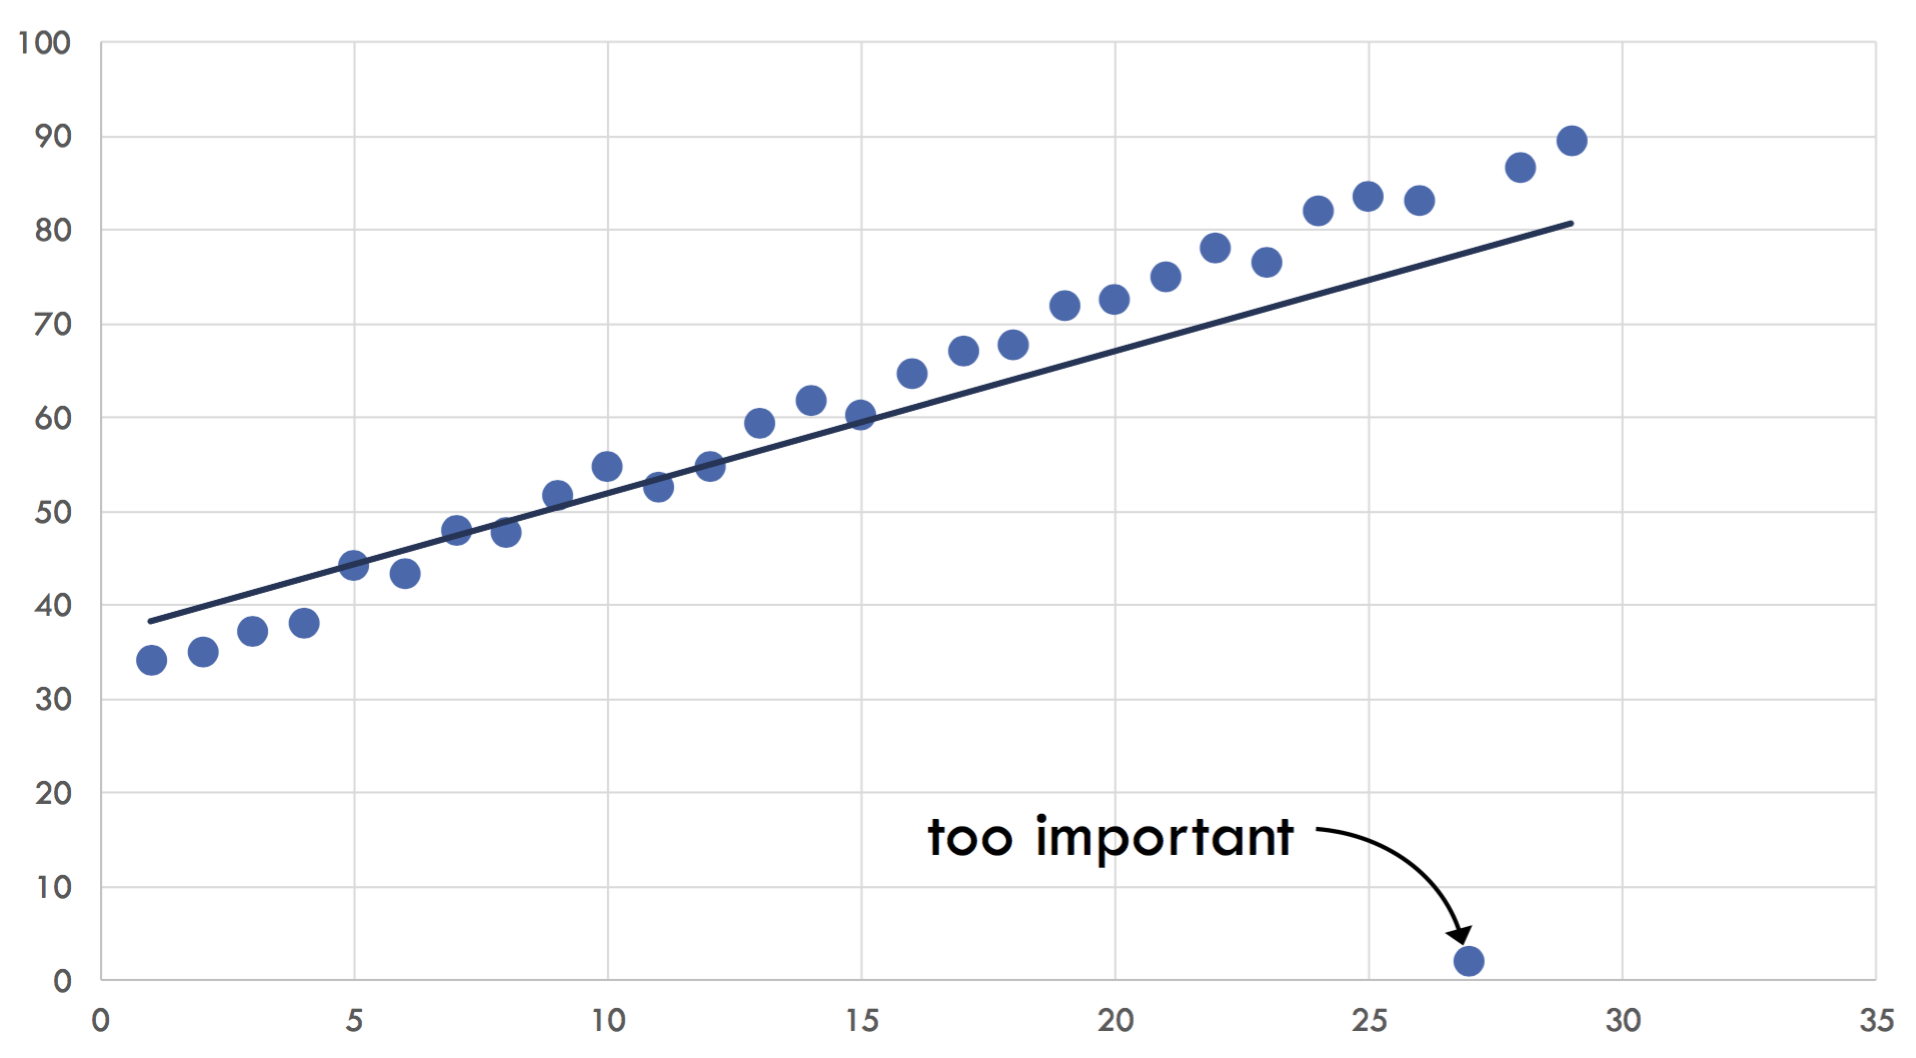
\includegraphics[scale=0.32]{pics/lpo.png}

\end{frame}

\subsection{}
\begin{frame}


  \frametitle{Outlier Penalty}

  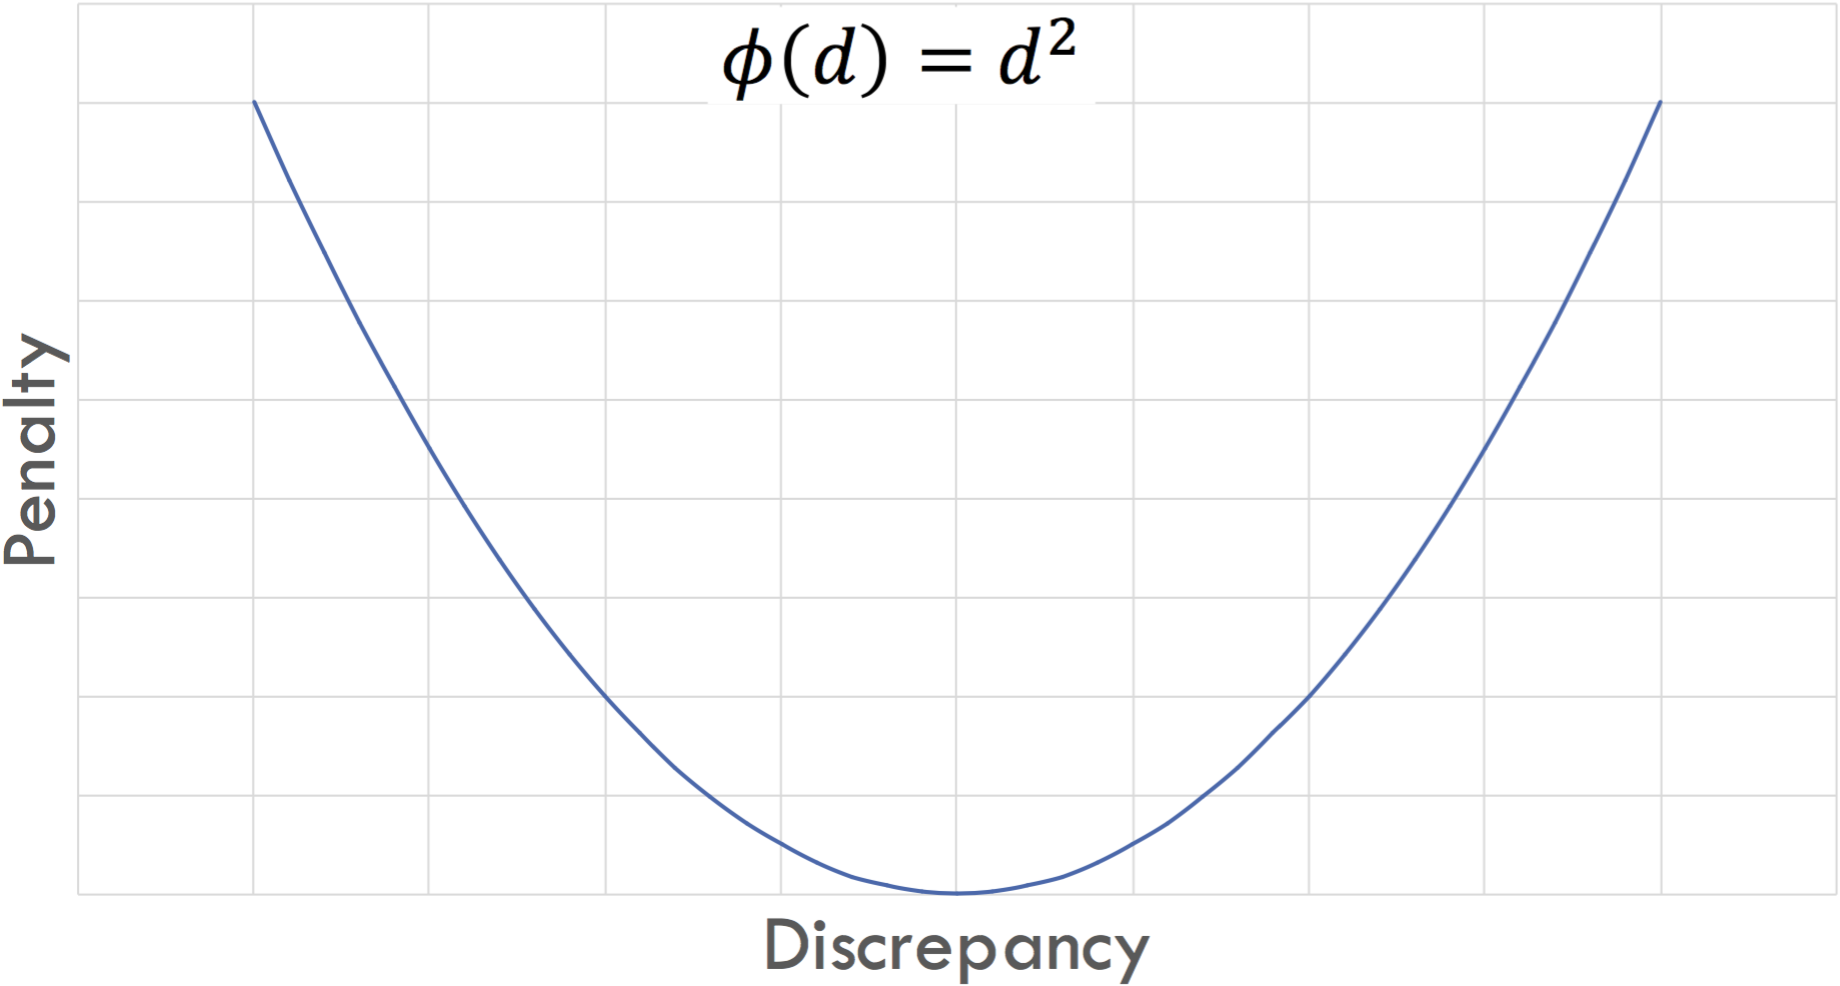
\includegraphics[scale=0.32]{pics/pen1.png}


\end{frame}

\begin{frame}
  \frametitle{Capped Penalty}
  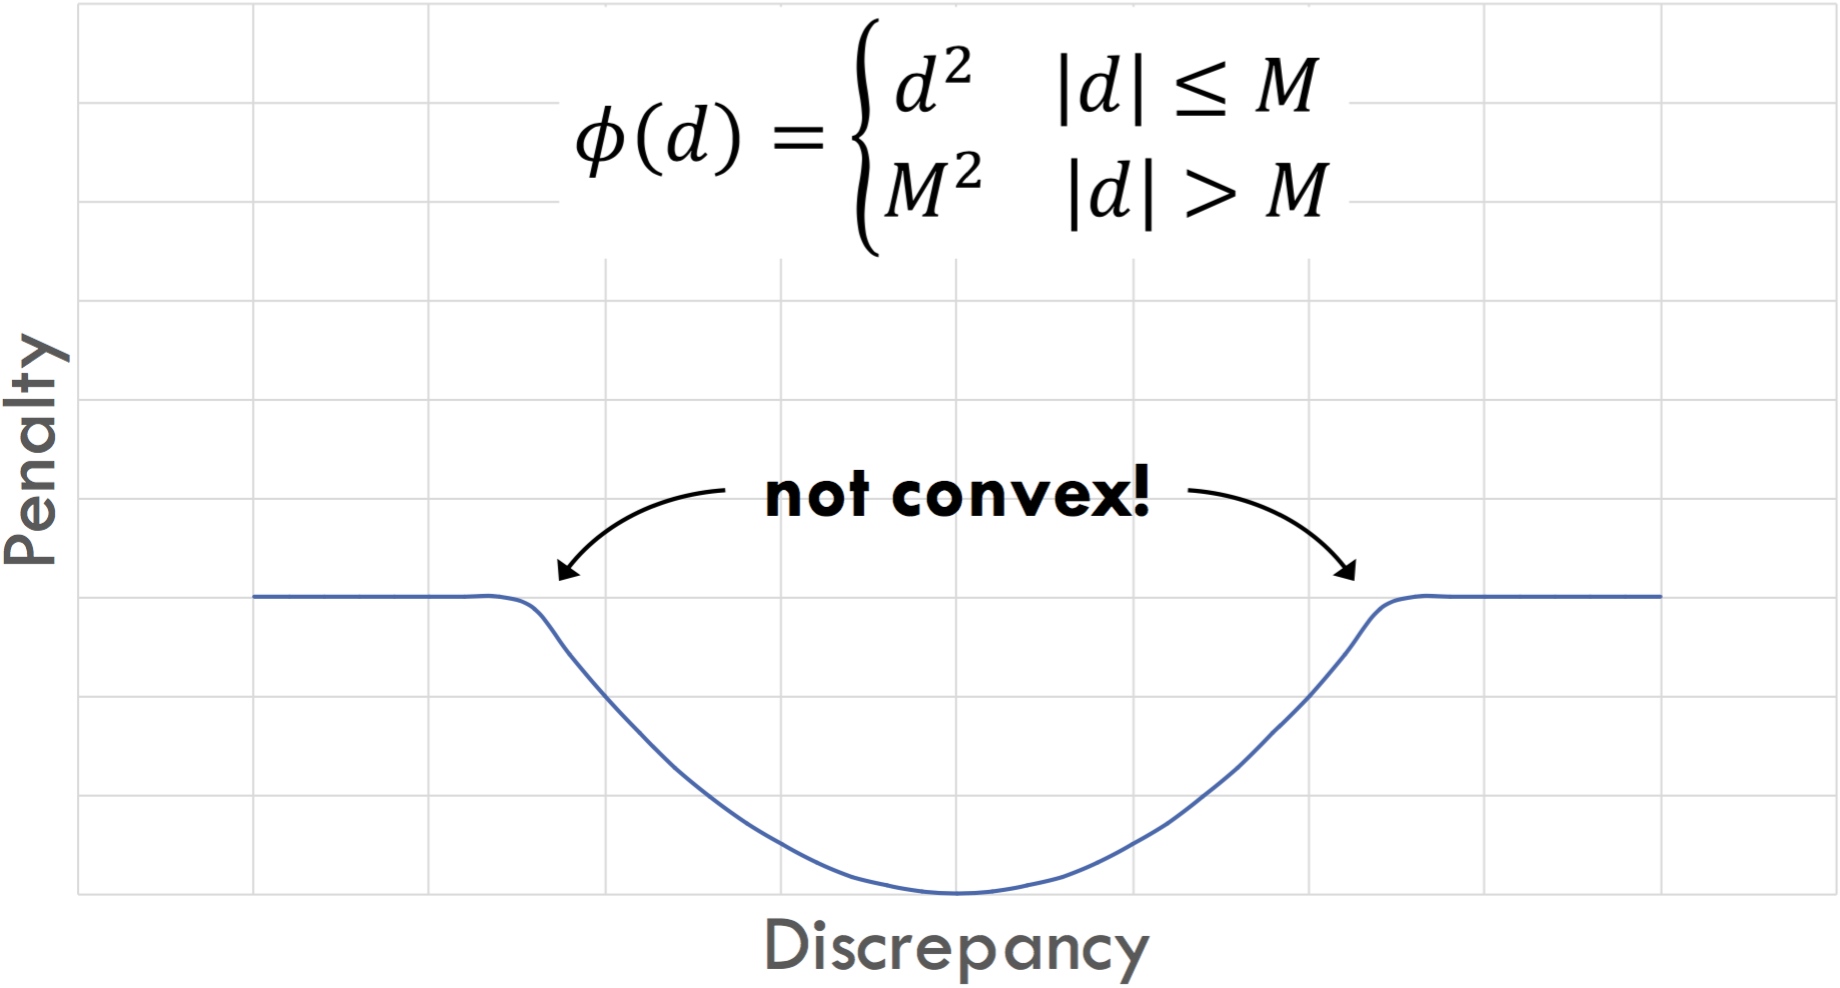
\includegraphics[scale=0.32]{pics/pen2.png}
\end{frame}

\begin{frame}
\frametitle{Huber Penalty Function}
  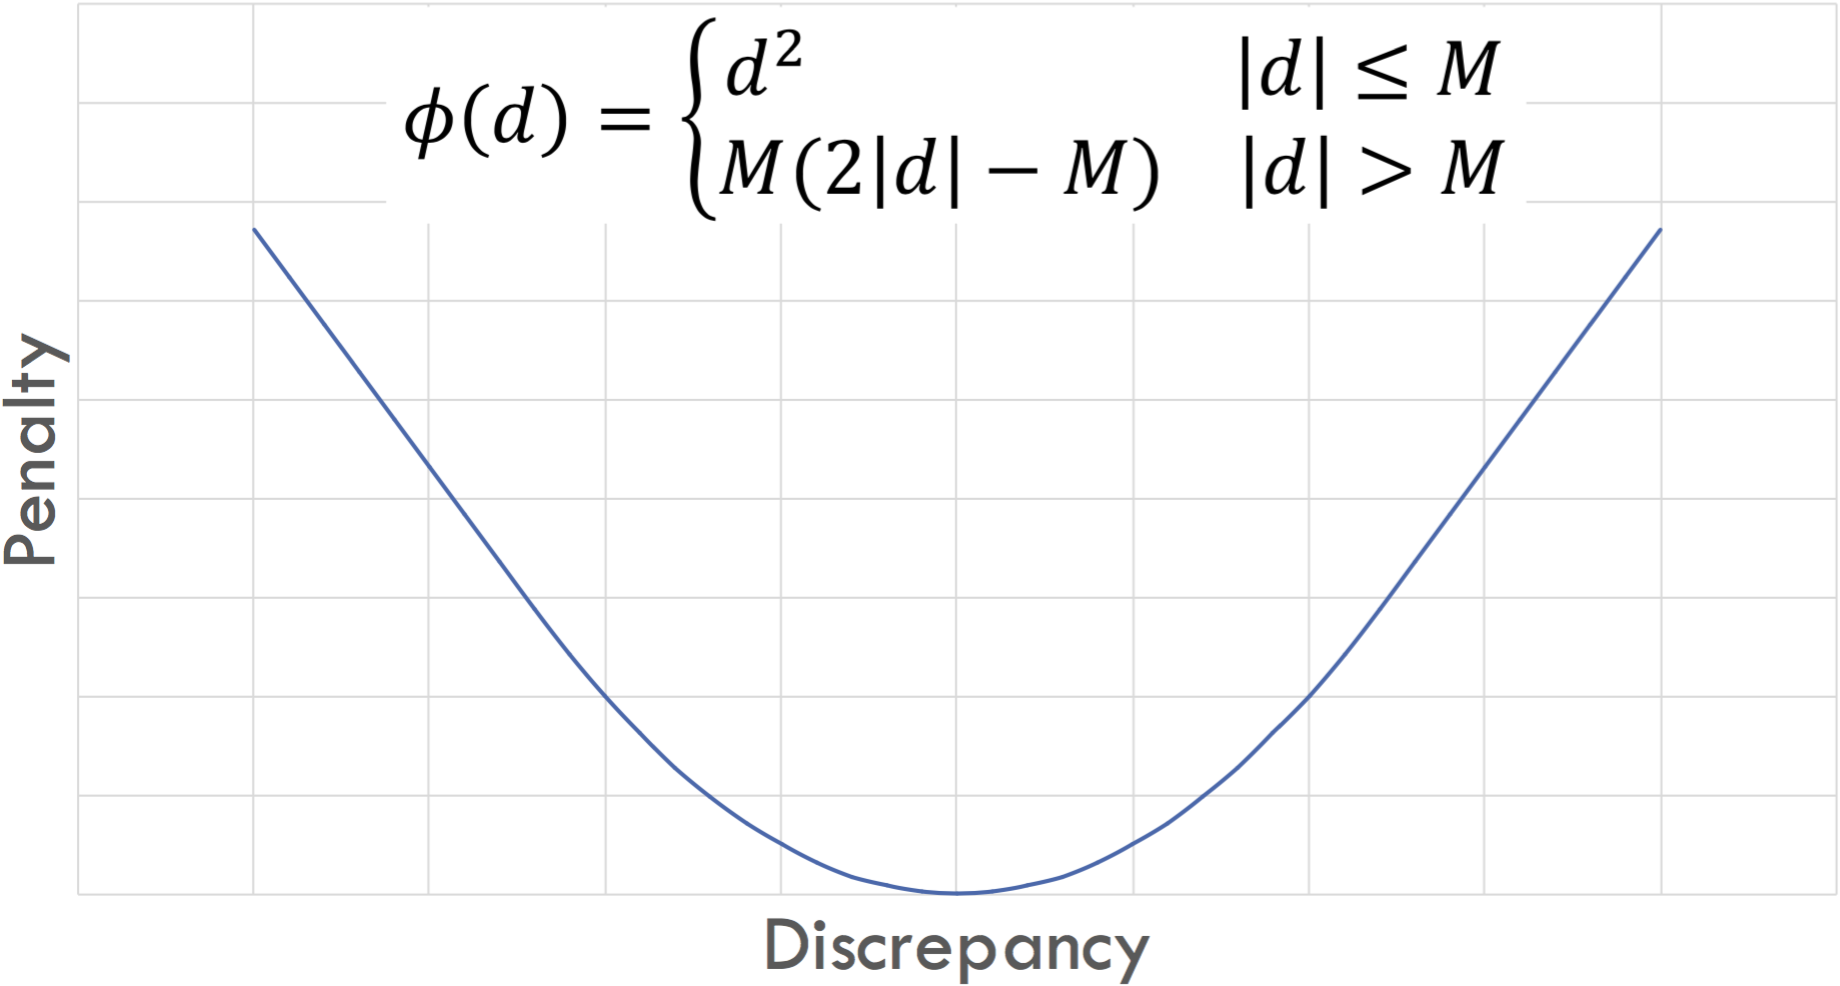
\includegraphics[scale=0.32]{pics/pen3.png}
\end{frame}




\section{Unconstrained Optimization}
%%% Local Variables:
%%% mode: latex
%%% TeX-master: t
%%% End:


\newcommand\desmeth{x^{(k+1)} = x^{(k)} + t^{(k)}\Delta x^{(k)}}
\newcommand\satis{{\bf \small s.t}.   f(x^{(k+1)}) < f(x^{(k)})}
\newcommand\xk[1]{x^{(#1)}}
\newcommand\bx{{\bf x}}

\subsection{}
\begin{frame}
  \frametitle{Unconstrained Optimization}
  \begin{itemize}
  \item Minimize $f(x)$;
  \item Where $f : \mathbb{R}^n \rightarrow \mathbb{R}$ is convex
    and twice differentiable;
  \item No additional constraints;
  \item Assume that unique minimum $x^*$ exists.
  \end{itemize}
\end{frame}

\begin{frame}
  \frametitle{General Principle}
  \begin{itemize}
  \item Objective: minimize $f(x)$
  \item Necessary and sufficient condition: $\nabla f(x^*) = 0$
    \begin{itemize}
    \item Solve analytically
    \item Iterative algorithms
    \end{itemize}
  \end{itemize}

  \begin{block}{ Iterative Algorithm:}
    $$\xk{0}, \xk{1}, ... \in \dom f$$
    $$k \rightarrow \infty, f(\xk{k}) \rightarrow f(x^*) $$
  \end{block}

  \begin{block}{Descent Method:}
    $$\desmeth,  \satis$$
  \end{block}

\end{frame}


\begin{frame}
  \frametitle{General Descent Method}
  \begin{block}{Descent Method:}
    \begin{equation}
      \desmeth,  \satis
      \label{equation: descent}
    \end{equation}
  \end{block}

  \only<1>{
    \begin{greenblock}{Algorithm:}
      \begin{algorithm}[H]
        \small
        Given $\xk{0} \in \dom f$\;
        \Repeat{stopping criterion is satisfied}{
          Determine a descent direction $\Delta x$\;
          Choose a step size $t > 0$\;
          Update $x := x + t \Delta x$\;
        }
        % \caption{Descent Method Algorithm}
      \end{algorithm}
    \end{greenblock}
  }

  \only<2>{
    \begin{greenblock}{Theorem}
      \footnotesize
      For a continuously differentiable function $f$:
      $$f~ is~ convex \Leftrightarrow f(x) \ge f(y) + f'(y)(x - y)$$
    \end{greenblock}
    \vspace{-8pt}
    \begin{greyblock}{Based on the Theorem and Equation (1):}
      \footnotesize
      $$ f(\xk{k}) + \nabla f(\xk{k})^T\Delta \xk{k} \le f(\xk{k+1}) $$
      $$\nabla f(\xk{k})^T\Delta \xk{k} \le f(\xk{k+1}) - f(\xk{k}) < 0$$

    \end{greyblock}
  }

  \only<3>{
    \begin{greenblock}{Algorithm:}
      \begin{algorithm}[H]
        \small
        \Repeat{G has 2 vertices}{
          {\bf choose} an edge $(v, w)$ uniformly at random from G\;
          {\bf let} $G\leftarrow \frac{G}{(v,w)}$
        }
        % \caption{Descent Method Algorithm}
      \end{algorithm}
    \end{greenblock}
  }


  \begin{block}{Therefore, $\Delta x$ must satisfy:}
    \begin{equation}
      \label{eq:xconv}
      \nabla f(\xk{k})^T\Delta \xk{k} < 0
    \end{equation}
  \end{block}
\end{frame}




\begin{frame}
  \frametitle{Line Search}

  \only<1>{
    $\desmeth, f(\xk{k+1}) \leftarrow f(\xk{k})$
    \begin{columns}
      \begin{column}{0.5\textwidth}
        \centering
        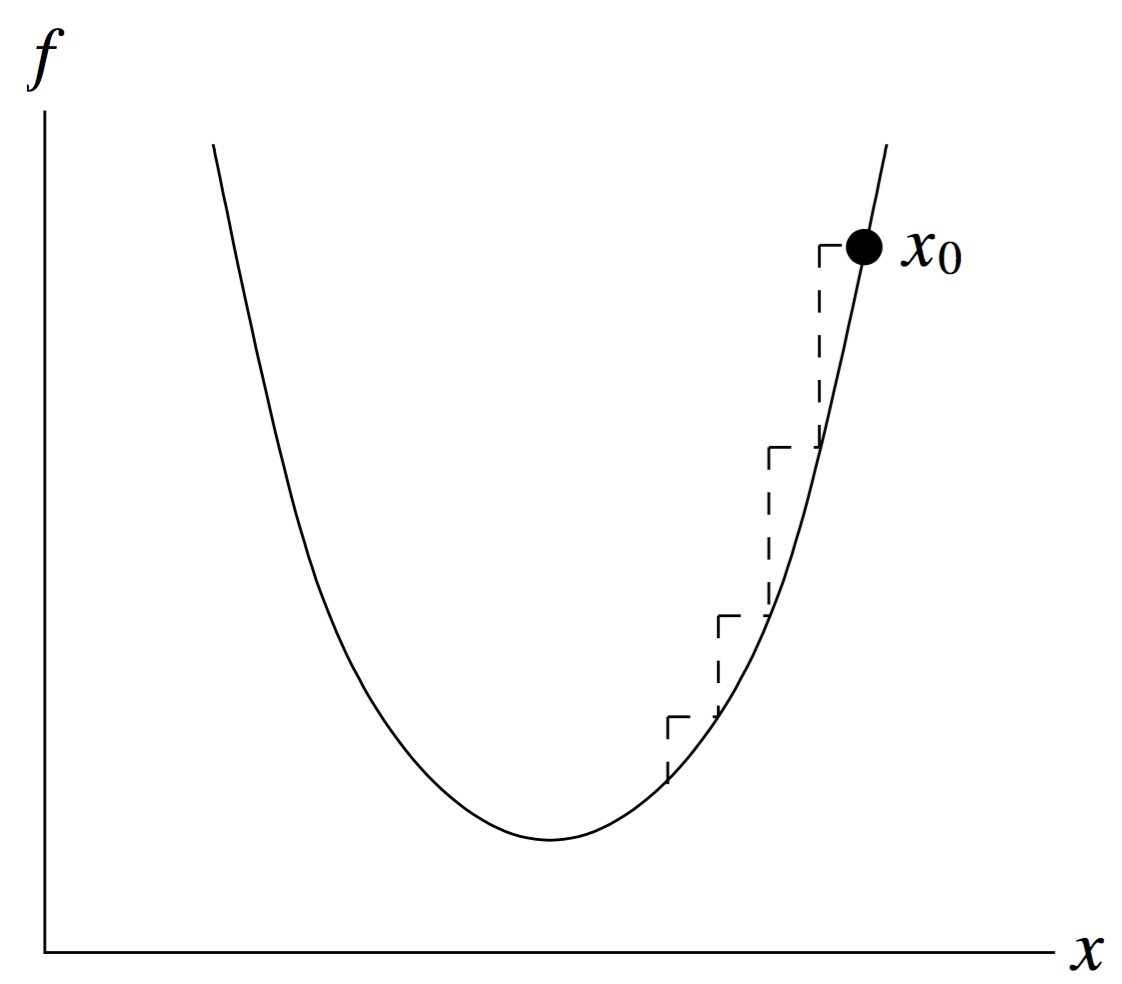
\includegraphics[scale=0.15]{pics/sa.png}

        {\tiny When Step Size t is Appropriate.}

        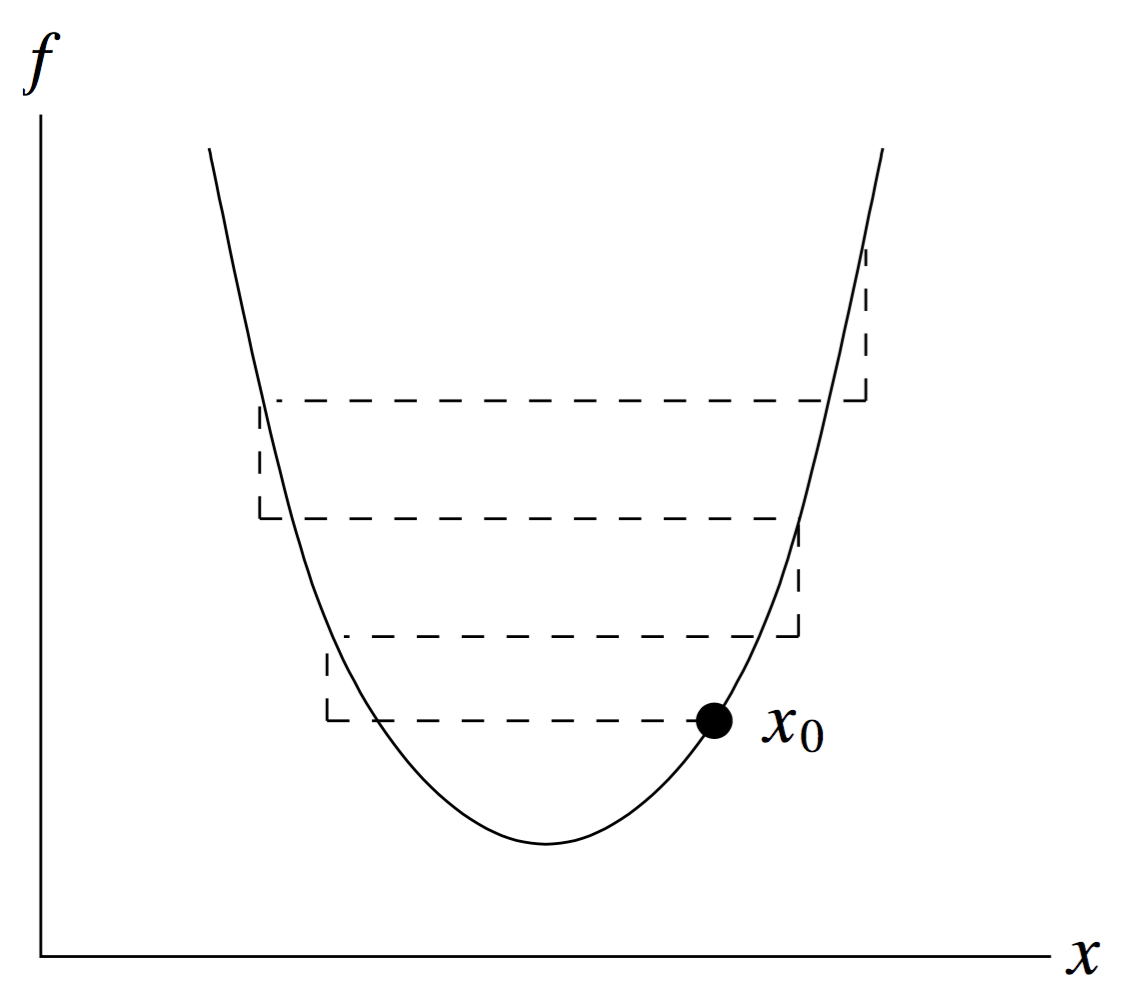
\includegraphics[scale=0.15]{pics/si.png}

        {\tiny When Step Size t is Inappropriate. }
      \end{column}


      \begin{column}{0.5\textwidth}
        \centering
        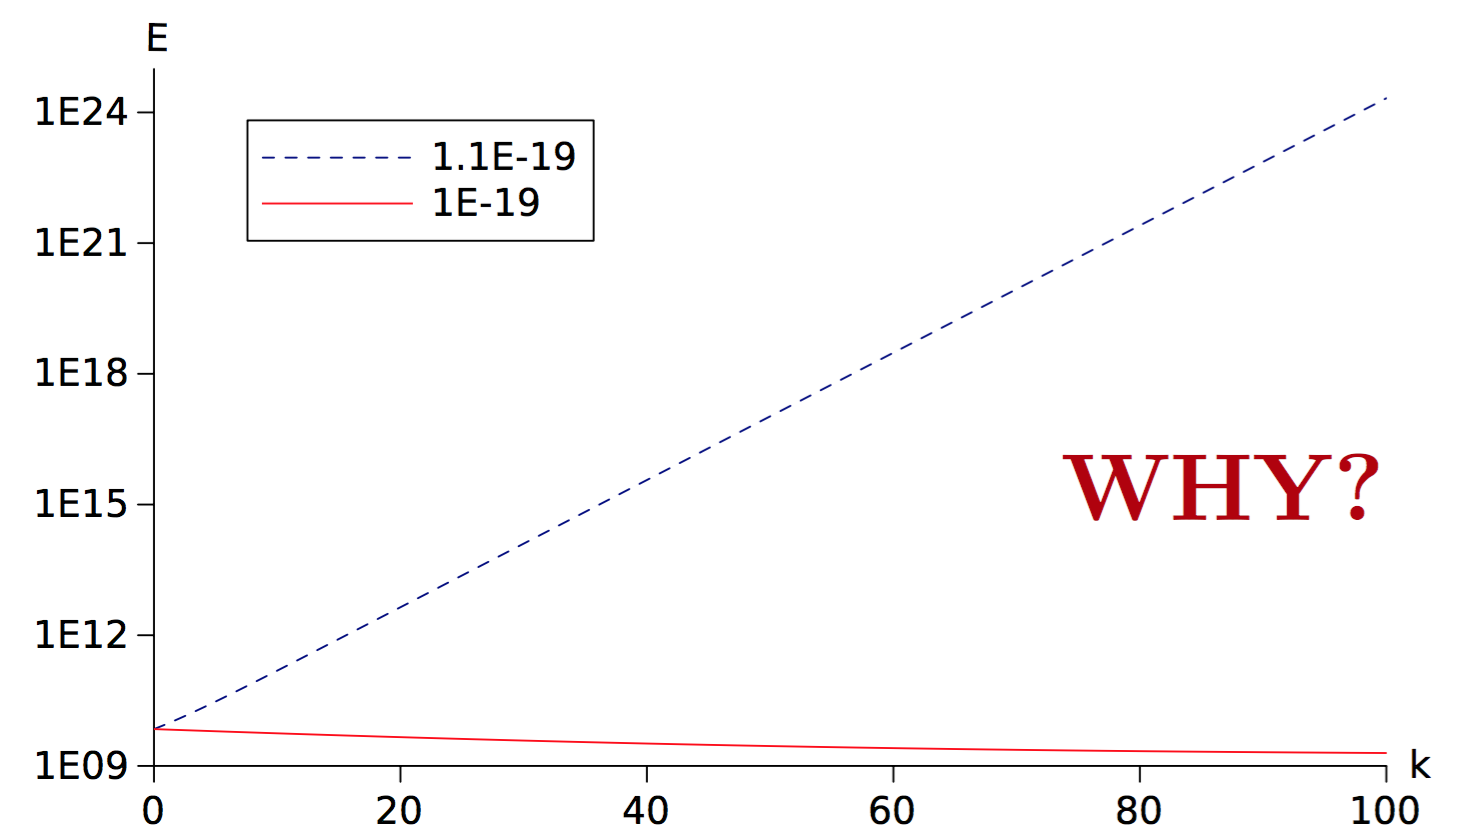
\includegraphics[scale=0.18]{pics/issue1.png}

        \vspace{4mm}

        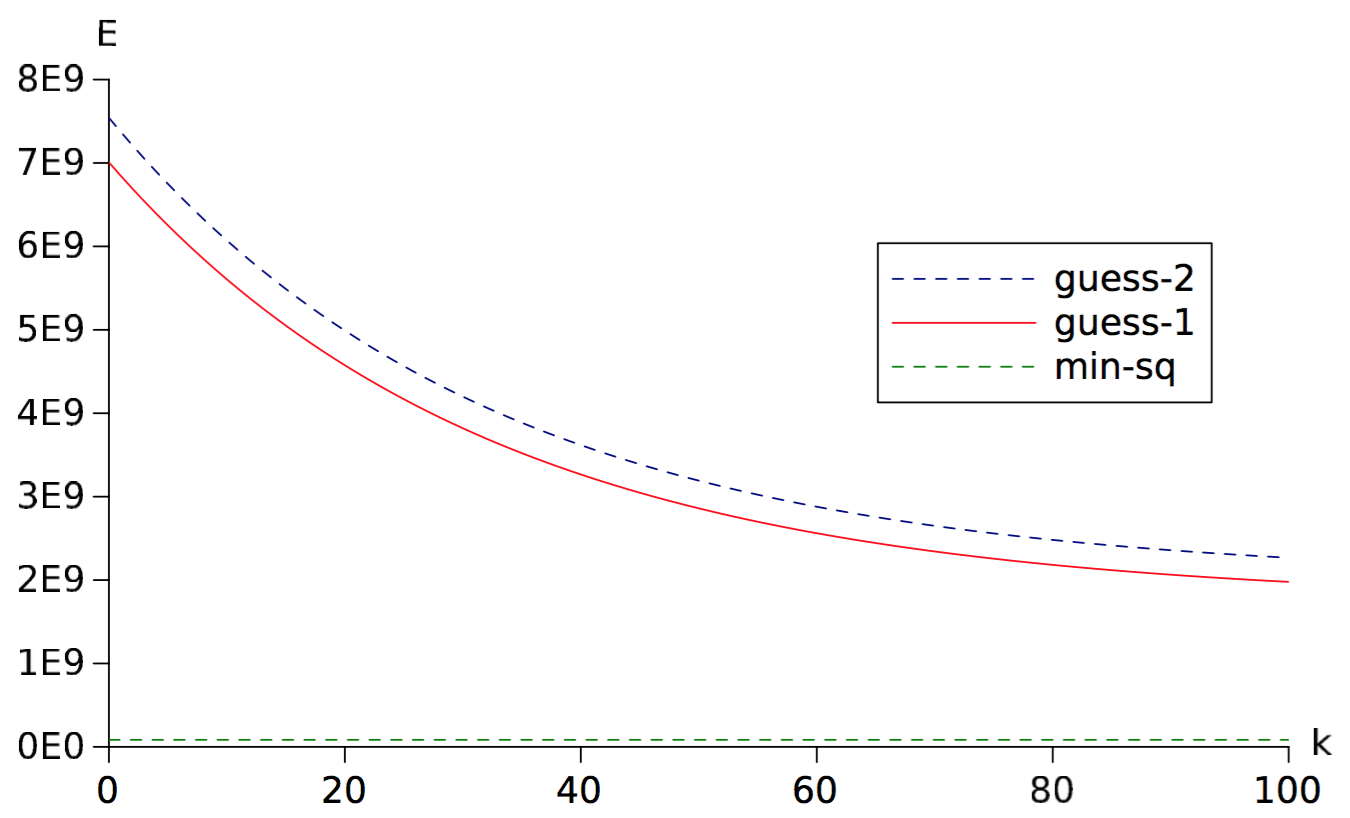
\includegraphics[scale=0.18]{pics/issue2.png}

      \end{column}
    \end{columns}
  }

  \only<2>{
    \begin{itemize}
    \item Armijo
      $$f(\xk{k} + t \Delta x^{(k)}) \le f(\xk{k}) + \alpha_1 t\nabla
      f(\xk{k})^T \Delta x^{(k)}, \alpha_1 > 0$$
    \item Wolfe Conditions (Including Armijo Condition):
      $$\nabla f(\xk{k} + t \Delta x^{(k)})^T\Delta x^{(k)} \ge
      \alpha_2\nabla f(\xk{k})^T\Delta x^{(k)}, 0< \alpha_1 < \alpha_2 < 1$$
    \end{itemize}

Where $\Delta x$ is the step direction.

    \begin{greenblock}{Theorem:}
      Gradient descent will find local minimum if step size $t$ satisfies Wolfe conditions.

    \end{greenblock}
  }

  \only<3>{
    \begin{itemize}
    \item Armijo Condition:
      $$f(\xk{k} + t\Delta \xk{k}) \le f(\xk{k}) + \alpha t\nabla
      f(\xk{k})^T\Delta \xk{k}, \alpha > 0$$
    \end{itemize}
    \begin{greenblock}{Backtracking Line Search:}
      \begin{algorithm}[H]
        \small
        Given a descent direction $\Delta x$ for $f$ at $x\in \dom f,
        \alpha \in (0, 0.5), \beta \in (0, 1), t := 1$\;
        \While{$f(x + t\Delta x) > f(x) + \alpha t\nabla
          f(x)^T\Delta x$}{
          $t :=\beta t$\;
        }
        % \caption{Descent Method Algorithm}
      \end{algorithm}
    \end{greenblock}
  {Exact Line Search Method:}
  $$\dis t = \argmin_{s\ge 0}\{f(x + s\Delta x)\} $$
  }


\end{frame}

\begin{frame}
  \frametitle{General Descent Method}
  \begin{itemize}
  \item Gradient Descent Method
  \item Steepest Descent Method
  \end{itemize}
  $\Delta x$ satisfies:
  $$\nabla f(\xk{k})^T\Delta \xk{k} < 0$$

\end{frame}


\begin{frame}
  \frametitle{Gradient Descent Method}
  \begin{greenblock}{$\Delta x = -\nabla f(x)$}
    \begin{algorithm}[H]
      \small
      Given $\xk{0} \in \dom f$\;
      \Repeat{stopping criterion is satisfied}{
        $\Delta x = -\nabla f(x)$\;
        Choose a step size $t > 0, [Line Search]$\;
        Update $x := x + t\Delta x$\;
      }
      % \caption{Descent Method Algorithm}
    \end{algorithm}
  \end{greenblock}
\end{frame}

\begin{frame}
  \frametitle{Steepest Descent Method}
  % Determine a descent direction $\Delta x$

  \only<1>{
    $\Delta x = \Delta x_{sd}$

    \textbullet Taylor Series:

    $$f(\bx + \Delta \bx) = f(\bx) + \nabla f(\bx)^T\Delta \bx +
    \frac{1}{2}\Delta\bx\nabla^2 f(\bx)\Delta \bx + ...$$

    $$f(\bx + {\bf v}) \approx \hat{f}(\bx + {\bf v}) = f(\bx) + \nabla
    f(\bx)^T{\bf v}$$

    $$\desmeth, \satis$$

    Where ${\bf v} $ is a descent direction if $\nabla f(\bx)^T{\bf v} < 0$
  }

  \only<2>{

    $$f(\bx + {\bf v}) \approx \hat{f}(\bx + {\bf v}) = f(\bx) + \nabla
    f(\bx)^T{\bf v}$$

    \textbullet Normalized Steepest Descent Direction:
    \begin{equation}
      \begin{split}
        \Delta \bx_{nsd} & = \argmin\{\nabla f(\bx)^T{\bf v}  ~| \norm{\bf v} = 1\} \\
        & =  \argmin\{\nabla f(\bx)^T{\bf v}  ~| \norm{\bf v} \le 1\}
      \end{split}
    \end{equation}

  }

  \only<3>{
    Dual Norm, denoted $\norm{\cdot}_*$, is defined as:
    $$\norm{z}_* = sup\{z^Tx | \norm{x}\le 1\}$$

    Unnormalized Steepest Descent Direction:
    $$\Delta \bx = \norm{\nabla f(x)}_* \cdot \Delta \bx_{nsd}$$
    \begin{columns}
      \begin{column}{0.4\textwidth}
        \footnotesize
        \begin{equation*}
          \label{eq:some}
          \begin{split}
            \nabla f(\bx)^T{\bf v} & = \nabla f(\bx)^T\Delta\bx_{sd} \\
            & =\norm{\nabla f(x)}_*\nabla f(\bx)^T\Delta\bx_{nsd} \\
            & = -\norm{\nabla f{(x)}}^2_*
          \end{split}
        \end{equation*}
      \end{column}
      \begin{column}{0.6\textwidth}
        \footnotesize
        \begin{greenblock}{Proof}
          \begin{equation*}
            \begin{split}
              \Delta \bx_{nsd} & = \argmin\{\nabla f(\bx)^T{\bf v} ~| \norm{v} \le 1\} \\
              & = - \argmax\{\nabla f(\bx)^T{\bf v} ~| \norm{v} \le 1\}
            \end{split}
          \end{equation*}
          \begin{equation*}
            \begin{split}
              \norm{\nabla f{(x)}}_* & = sup\{\nabla f(\bx)^T{\bf v}~ |
              \norm{v} \le 1 \} \\
              \Rightarrow \norm{\nabla f{(x)}}_* & = -\nabla f(\bx)^T\Delta x_{nsd}
            \end{split}
          \end{equation*}
        \end{greenblock}
      \end{column}
    \end{columns}

  }

  \only<4>{
    $\Delta \bx_{nsd}  = \argmin\{\nabla f(\bx)^T{\bf v}~ | \norm{\bf v} \le
    1\}$

    $\Delta \bx_{sd} = \norm{\nabla f(\bx)}_*\Delta \bx_{nsd}$

    \begin{greenblock}{Steepest Descent Method}
      \begin{algorithm}[H]
        \small
        Given $x \in \dom f$\;
        \Repeat{
        stopping criterion is satisfied}{
          Compute steepest descent direction $\Delta x_{sd}$\;
          Choose a step size $t > 0, [Line Search]$\;
          Update $x := x + t\Delta x_{sd}$\;
        }
        % \caption{Descent Method Algorithm}
      \end{algorithm}
    \end{greenblock}

When exact line search is used, scale factors in the descent direction have no effect.
  }

\end{frame}



\begin{frame}
  \frametitle{Descent Method}

\only<1>{
  \begin{blueblock}{General}
    \begin{algorithm}[H]
      \tiny
      Given $x \in \dom f$\;
      \Repeat{ stopping criterion is satisfied}{
        Determine a descent direction $\Delta x$\;
        Choose a step size $t > 0$\;
        Update $x := x + t\Delta x$\;
      }
      % \caption{Descent Method Algorithm}
    \end{algorithm}
  \end{blueblock}
}

\only<2>{
  \begin{blueblock}{General}
  \begin{itemize}
  \item $\Delta \bx_{nsd}  = \argmin\{\nabla f(\bx)^T{\bf v} ~| \norm{\bf v} \le
    1\} $
  \item $\Delta\bx_{sd} = \norm{\nabla f(x)}_*\cdot \Delta \bx_{nsd}$
  \item If the norm $\norm{\cdot}$ is Euclidean norm, $\Delta \bx =
    -\nabla f(\bx)$, which means that Gradient Descent and Steepest
    Descent become the same.
  \end{itemize}
  \end{blueblock}
\vspace{2mm}

}


  \begin{columns}[t]
    \begin{column}{0.5\textwidth}
      \begin{greenblock}{Gradient Descent}
        \begin{algorithm}[H]
          \tiny
          Given $x \in \dom f$\;
          \Repeat{
            stable  stopping criterion is satisfied}{
          $\Delta x = -\nabla f(x)$\;
          Choose a step size $t > 0, [Line Search]$\;
          Update $x := x+ t\Delta x$\;
        }

        \end{algorithm}

      \end{greenblock}
    \end{column}

    \begin{column}{0.5\textwidth}
      \begin{greenblock}{Steepest Descent}
        \begin{algorithm}[H]
          \tiny
          Given $x \in \dom f$\;
          \Repeat{
            stable stable  stopping criterion is satisfied}{
          Compute steepest descent direction $\Delta x_{sd}$\;
          Choose a step size $t > 0, [Line Search]$\;
          Update $x := x + t\Delta x_{sd}$\;
        }


        \end{algorithm}
        %   \small
        %   Given $\xk{0} \in \dom f$\;
        %   \Repeat{$\Delta x$ is within an acceptable range and is stable;}{
        %   Compute steepest descent direction $\Delta x_{sd}$\;
        %   Choose a step size $t > 0, [Line Search]$\;
        %   Update $x^{(k+1)} = x^{(k)} + t^{(k)}\Delta x^{(k)}_{sd}$\;
        % }

      \end{greenblock}

    \end{column}

  \end{columns}

\end{frame}

% \begin{frame}
%   \frametitle{Steepest Descent Method}
%   \begin{block}
%     \begin{algorithm}[H]
%       \small
%       Given $\xk{0} \in \dom f$\;
%       \Repeat{$\Delta x$ is within an acceptable range and is stable}{
%       Determine a descent direction $\Delta x$\;
%       Choose a step size $t > 0$\;
%       Update $\desmeth$\;
%     }
%       %       \caption{Descent Method Algorithm}
%     \end{algorithm}
%   \end{block}

%   \begin{columns}
%     \begin{column}{0.5\textwidth}
%       \begin{greenblock}
%         \begin{algorithm}[H]
%           \small
%           Given $\xk{0} \in \dom f$\;
%           \Repeat{$\Delta x$ is within an acceptable range and is stable}{
%           $\Delta x = -\nabla f(\xk{k})$\;
%           Choose a step size $t > 0, [Line Search]$\;
%           Update $x^{(k+1)} = x^{(k)}+ t\Delta x$\;
%         }

%         \end{algorithm}
%       \end{greenblock}
%     \end{column}

%     \begin{column}{0.5\textwidth}
%       \begin{greenblock}
%         \begin{algorithm}[H]
%           \small
%           Given $\xk{0} \in \dom f$\;
%           \Repeat{$\Delta x$ is within an acceptable range and is stable;}{
%           Compute steepest descent direction $\Delta x_{sd}$\;
%           Choose a step size $t > 0, [Line Search]$\;
%           Update $x^{(k+1)} = x^{(k)} + t^{(k)}\Delta x^{(k)}_{sd}$\;
%         }

%         \end{algorithm}
%       \end{greenblock}
%     \end{column}

%   \end{columns}

% \end{frame}

%%% Local Variables:
%%% mode: latex
%%% TeX-master: t
%%% End:


\section{Convex Domain}
%%% Local Variables:
%%% mode: latex
%%% TeX-master: t
%%% End:


\section{Applications}
%%% Local Variables:
%%% mode: latex
%%% TeX-master: t
%%% End:

\newenvironment<>{redblock}[1]{%
  \setbeamercolor{block title}{fg=white,bg=red!75!black!65}%
  \setbeamercolor{block body}{fg=red!40!black!70,bg=red!60!black!20}%

  \begin{block}#2{#1}}{\end{block}}
\newenvironment<>{blueblock}[1]{%
  \setbeamercolor{block title}{fg=white,bg=blue!75!black!65}%
  \setbeamercolor{block body}{fg=black,bg=blue!60!black!20}%
  \begin{block}#2{#1}}{\end{block}}

\newenvironment<>{greyblock}[1]{%
  \setbeamercolor{block title}{fg=white,bg=black!75}%
  \setbeamercolor{block body}{fg=black,bg=black!40}%
  \begin{block}#2{#1}}{\end{block}}


\section{Applications}

\subsection{Image Processing}

\begin{frame}
\frametitle{Image Processing --- Lucas-Kanade}
  \begin{itemize}
  \item[] {
Classic examples are optical flow techniques like Lucas-Kanade (VideoTracking), Horn-Schunck.
  }
  \end{itemize}


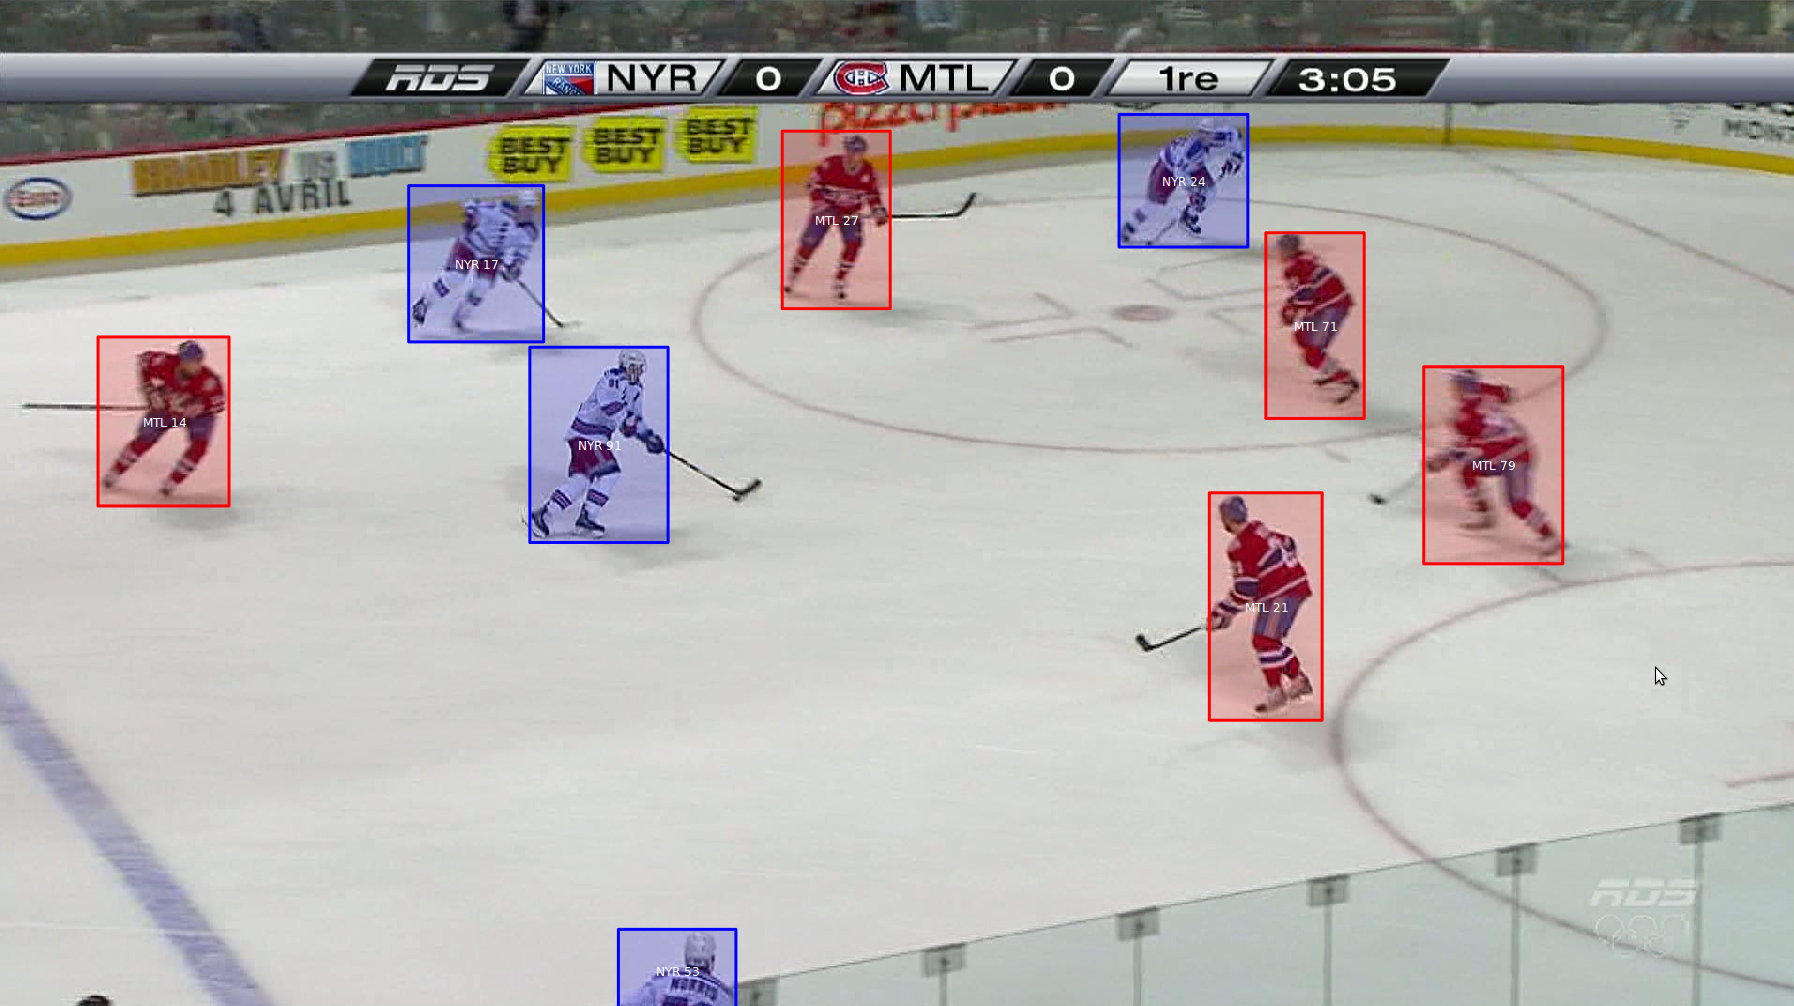
\includegraphics[scale=0.15]{right2.png}
\end{frame}

\begin{frame}
\frametitle{Lucas-Kanade}

\begin{blueblock}{Goal of Lucas-Kanade}
Minimize the sum of squared error between two images.
\end{blueblock}

\begin{redblock}{Assumption}
The displacement of the image contents between two nearby instants
(frames) is small and approximately constant within a neighborhood of
the point $p$ under consideration.
\end{redblock}

\end{frame}

\begin{frame}
\frametitle{Lucas-Kanade}
  \begin{blueblock}{Optical Flow Equation (2 Dementional)}
For a pixel location $(x, y, t)$, the intensity has moved by $\Delta
x, \Delta y, \Delta t$, the basic assumption can be represented as:
$$I(x, y, t) = I(x + \Delta x, y + \Delta y, t + \Delta t)$$

  \end{blueblock}
\end{frame}

\begin{frame}
\frametitle{Lucas-Kanade}
  \begin{blueblock}{Optical Flow Effect:}
For all pixels within a window centered at p:
$$I_x(q_i)V_x + I_y(q_i)V_y = -I_t(q_i) $$
Where  $i = 1,2,3 ... n$.

  \end{blueblock}

  \begin{greyblock}{Abbreviations:}
$$ A = [ I_x(q_i)^T, I_y(qi)^T] $$
$$ V = [v_x, v_y]^T $$
$$ b = [-I_t(q_i)]^T $$
  \end{greyblock}
\end{frame}

\begin{frame}
\frametitle{Lucas-Kanade}
  \begin{blueblock}{Lucas-Kanade Method Abstraction:}
LK method tries to solve $2 \times 2$ system:
$$A^TAV = A^Tb$$

A.K.A:

$$V = (A^TA)^{-1}A^Tb$$
  \end{blueblock}

  \begin{greyblock}{Notice:}
    $V = [v_x, v_y]^T$ is variable. Which means that the system does
    not know the actual velocity of the system.
  \end{greyblock}
\end{frame}


\begin{frame}
\frametitle{Lucas-Kanade}
  \begin{blueblock}{Goal of Lucas-Kanade Method:}
To minimize $||A^TV - b||^2$.
  \end{blueblock}
Basic LK Derivation for Models(Stuff to be Tracked):
$$E[v_x, v_y] = \Sigma [I(x+v_x, y+v_y) - T(x, y)]^2$$
Where $v_x, v_y$ is the hypothesized location of the model(s) to be
tracked, and $T(x, y)$ model.
\end{frame}

\begin{frame}{ \LARGE APPLICATIONS -- IMAGE PROCESSING}
\frametitle{Lucas-Kanade}
  \begin{redblock}{Key Step for Implementation of GD (Step 1):}
    Generalizing LK approach by introducing warp function W:
    $$E[v_x, v_y]  = \Sigma [I(W(x, y); P) - T(x,y)]^2$$
    Generalizing is used to solve the problem where the constant flow
    of larger picture frames for a long time is a total waste of
    calculation power. Warp function examples are {\bf Affine}  and
    {\bf Projective}. \\
The warping function are the {\bf convergence factor} for steepest descent
algorithm.
  \end{redblock}
\end{frame}


\begin{frame}
\frametitle{Lucas-Kanade}
  \begin{redblock}{Key Step for Implementation of GD (Step 2):}
The key to the derivation is Taylor series approximation:
$$ I(W(x, y); P + \Delta P) \approx I(W([x, y]; P)) + \nabla I
\frac{\partial W}{\partial P}\Delta P$$
  \end{redblock}

\begin{itemize}
\item The approximation equation is actually the abstract of the basic
assumption of optical flow described in the slides before.
\item Derivation of this equation can be discussed in forum (Too long
  for slides).

\end{itemize}




\end{frame}

\begin{frame}
\frametitle{Lucas-Kanade}
  \begin{blueblock}{Some Explainations:}
    \begin{itemize}
\item Gradient image $\nabla I$
\item Image error $I_E = T(x, y) - I(W[x, y]; P)$
\item Jacobian matrix $ \frac{\partial W}{\partial P} $
\item Steepest image  $ I_S =  \nabla I \frac{\partial W}{\partial P}$
\item Hessian Matrix $\Sigma (\nabla I \frac{\partial W}{\partial
    P})^T(\nabla I \frac{\partial W}{\partial P})$
\item Iteration step $ \Delta P =  \Sigma I_S^T I_E$
    \end{itemize}

\end{blueblock}

\end{frame}

\begin{frame}
\frametitle{Lucas-Kanade}
  \begin{greyblock}{Algorithms: }
    \begin{itemize}
    \item Warp image and get $I(W[x, y]; P)$;
    \item Get image error $I_E$;
    \item Warp gradient image $\nabla I$;
    \item Evaluate Jacobian;
    \item Compute steepest descent image  $I_S = \nabla I \frac{\partial W}{\partial
    P}$;
    \item Compute Hessian matrix $\Sigma I_S^TI_S$;
    \item Get warping step $\Delta P = I_SI_E$;
    \item Update warping parameter $P = P + \Delta P$;
      \item Repeat until $\Delta P$ is negligible.
    \end{itemize}
  \end{greyblock}
\end{frame}


\subsection{MACHINE LEARNING}


\begin{frame}{ \LARGE APPLICATIONS -- MACHINE LEARNING}
  \begin{blueblock}{Generalized Utilization of Convex: Delta Rule}
\begin{itemize}
\item The delta rule is derived by attempting to minimize the error in the output of the neural network through gradient descent.
\item Gradient Descent optimization is the most basic principle for
  training neurons even with different activation functions.
\item Delta rule, can also be modified, if possible, with steepest descent method.
\end{itemize}
  \end{blueblock}

\end{frame}

\begin{frame}{ \LARGE APPLICATIONS -- MACHINE LEARNING}
  \begin{redblock}{Delta Rule:}
$$\Delta w_{ji} = \alpha (t_j - y_j)g'(h_j)x_j$$
Where $\alpha$ is the learning rate, $g(x)$ is the neuron's activation
function. $t_j$ and $y_j$ is the target and actual output of the
neuron. $h_j$ is the weighted sum of the neuron's inputs. And $x_i$ is
the $i_{th}$ input.
  \end{redblock}

  \begin{greyblock}{The above equation holds the following:}
$$h_j = \Sigma x_iw_{ji}$$
$$y_j = g(h_j)$$

  \end{greyblock}

\end{frame}

\subsection{ROBOTICS}
\begin{frame}{ \LARGE APPLICATIONS -- INVERSE KINEMATICS}
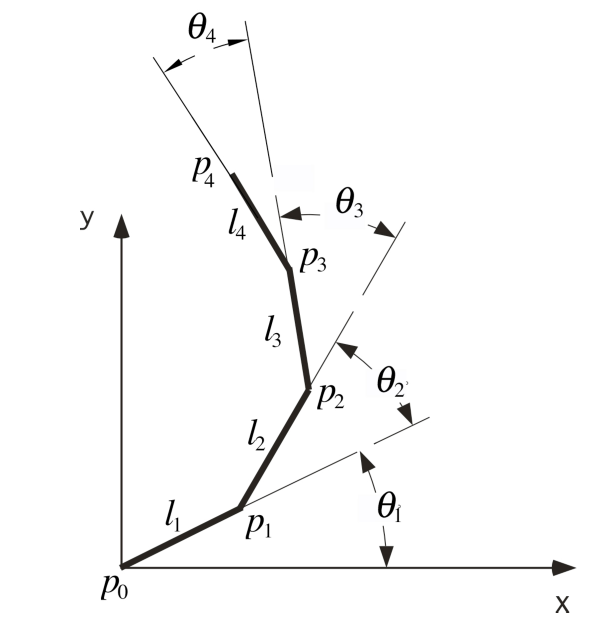
\includegraphics[scale=0.6]{jcob.png}

\end{frame}

\begin{frame}{ \LARGE APPLICATIONS -- INVERSE KINEMATICS}
  \begin{blueblock}{Goal of Inverse Kinematics}
Given a position in the space, calculate a way for a robot hand to reach a place.

  \end{blueblock}
  \begin{redblock}{Problem Abstract:}
$$\vec{e} = R_1T_1R_2T_2R_3T_3R_4T_4\vec{e_0}$$
 Where $T_i$ is a series of translation transformation and $R_i$ is a
 series of rotation translation.

  \end{redblock}

\end{frame}

\begin{frame}{ \LARGE APPLICATIONS -- INVERSE KINEMATICS}
  \begin{redblock}{Abstraction for Convex Optimization:}
$$\Delta \vec{\theta} = \alpha J^T \vec{e}$$.

The target for the optimization is to achieve $|\vec{e_p}-\vec{e_t}| =
0$, where $\vec{e_p}$ is th original position of the tip of the
robotic arm and $\vec{e_t}$ is the target position.
$J$ is the jacobian matrix in terms of $\vec{\theta}$, which is the
vector of all the spatial angles of all  joints. $\alpha$ is the
convergence rate and $\vec{e}$ is the position derivation (step size).

  \end{redblock}

\end{frame}

\begin{frame}{ \LARGE APPLICATIONS -- INVERSE KINEMATICS}
  \begin{greyblock}{About Inverse Kinematics}
    \begin{itemize}
    \item Jacobian transpose is the implementation of gradient descent
      in the real physical world.
    \item It can actually achieve {\bf near linear} solution for
      robotic arms with a fast convergence rate.
    \end{itemize}
  \end{greyblock}

\end{frame}


\section{References}
\begin{frame}
  \frametitle{References}
\tiny
\bibliographystyle{plain}
\bibliography{references}


\end{frame}




% \section{Section no. 2}
% \subsection{Lists I}
% \begin{frame}
%   \frametitle{unnumbered lists}
%   \begin{itemize}
%   \item Introduction to  \LaTeX{}
%   \item Course 2
%   \item Termpapers and presentations with \LaTeX{}
%   \item Beamer class
%   \end{itemize}
% \end{frame}

% \begin{frame}\frametitle{lists with single pauses}
%   \begin{itemize}
%   \item Introduction to  \LaTeX{}  \pause
%   \item Course 2 \pause
%   \item Termpapers and presentations with \LaTeX{}  \pause
%   \item Beamer class
%   \end{itemize}
% \end{frame}

% \begin{frame}\frametitle{lists with pause}
%   \begin{itemize}[<+->]
%   \item Introduction to  \LaTeX{}
%   \item Course 2
%   \item Termpapers and presentations with \LaTeX{}
%   \item Beamer class
%   \end{itemize}
% \end{frame}



% \subsection{Lists II}
% \begin{frame}\frametitle{numbered lists}
%   \begin{enumerate}
%   \item Introduction to  \LaTeX{}
%   \item Course 2
%   \item Termpapers and presentations with \LaTeX{}
%   \item Beamer class
%   \end{enumerate}
% \end{frame}

% \begin{frame}
%   \frametitle{numbered lists with single pauses}
%   \begin{enumerate}
%   \item Introduction to  \LaTeX{}  \pause
%   \item Course 2 \pause
%   \item Termpapers and presentations with \LaTeX{}  \pause
%   \item Beamer class
%   \end{enumerate}
% \end{frame}

% \begin{frame}
%   \frametitle{numbered lists with pause}
%   \begin{enumerate}[<+->]
%   \item Introduction to  \LaTeX{}
%   \item Course 2
%   \item Termpapers and presentations with \LaTeX{}
%   \item Beamer class
%   \end{enumerate}
% \end{frame}




% \section{Section no.3}
% \subsection{Tables}
% \begin{frame}
%   \frametitle{Tables}
%   \begin{tabular}{|c|c|c|}
%     \hline
%     \textbf{Date} & \textbf{Instructor} & \textbf{Title} \\
%     \hline
%     WS 04/05 & Sascha Frank & First steps with  \LaTeX  \\
%     \hline
%     SS 05 & Sascha Frank & \LaTeX \ Course serial \\
%     \hline
%   \end{tabular}
% \end{frame}


% \begin{frame}
%   \frametitle{Tables with pause}
%   \begin{tabular}{c c c}
%     A & B & C \\
%     \pause
%     1 & 2 & 3 \\
%     \pause
%     A & B & C \\
%   \end{tabular}
% \end{frame}


% \section{Section no. 4}
% \subsection{blocs}
% \begin{frame}
%   \frametitle{blocs}

%   \begin{block}{title of the bloc}
%     bloc text
%   \end{block}

%   \begin{exampleblock}{title of the bloc}
%     bloc text
%   \end{exampleblock}


%   \begin{alertblock}{title of the bloc}
%     bloc text
%   \end{alertblock}
% \end{frame}

\end{document}


%%% Local Variables:
%%% mode: latex
%%% TeX-master: t
%%% End:
